\chapter{Flashing the FPGAs and CPLDs in the MEGA65}
\label{cha:fpgacpldflashing}

The MEGA65 is an open-source and open-hardware computer. This means you are free,
not only to write programs that run on the MEGA65 as a finished computer, but you can
use the re-programmable chips in the MEGA65 to turn it into all sorts of other things!

If you just want to install an upgrade core for the MEGA65, or a core that lets you use
your MEGA65 as another type of computer, you are probably looking for
Chapter \ref{cha:cores} instead.
This chapter is more intended for people who want to help develop cores for the MEGA65.

These re-programmable chips are called Field Programmable Gate Arrays (FPGAs) or
Complex Programmable Logic Devices (CPLDs), and can implement a wide variety of circuits.
They are normally programmed using a programming language like VHDL or Verilog.  These
are languages that are not commonly encountered by most people.  They are also quite
different in some ways to ``normal'' programming languages, and it can take a while to
understand how they work, but with some effort and perseverance, many people will be
able to do exiting things with them.

Be prepared to install many gigabytes of software on a Linux or Windows PC, before you will
be able to write programs for the FPGAs and CPLDs in the MEGA65.  Also,
"compiling" complex
designs can take up to several hours, depending on the speed and memory
capacity of your computer!
We recommend a computer with at least 8GB RAM, and preferably 16GB if you want to write
programs for FPGAs and CPLDs. If on the other hand all you want to do is load programs onto
your MEGA65's FPGAs and CPLDs that other people have written, then most
computers running a recent
version of Windows or Linux should be able to cope.

\section{Warning}

Before we go any further, we do have to provide a warning about reprogramming the FPGAs and
CPLDs in the MEGA65.
Re-programming the MEGA65 FPGA can potentially cause
damage, or leave your MEGA65 in an unresponsive state from which it is very difficult to
recover, i.e., ``bricked''.  Therefore if you choose to open your MEGA65 and reprogram
any of the FPGAs it contains, it is no longer possible to guarantee its correct operation.
Therefore in this case we can not reasonably honour the warranty of the
device as a computer.
You have been warned!

\section{Flashing the Artix 100T main FPGA with XILINX VIVADO}

If you choose to proceed, you will need a TE0790-03 JTAG programming module, a functioning
installation of Xilinx's Vivado software.  This can be done on either Windows or Linux, but
in both cases you will need to install any necessary USB drivers. It is
also necessary to have
dip-switches 1 and 3 in the ON position and dip-switches 2 and 4 in the
OFF position on the TE-0790.
With your MEGA65 disconnected from the power, the TE-0790 must be
installed on the JB1 connector,
which is located between the floppy data cable and the audio jack.
The gold-plated hole of the TE-0790 must line up with the screw
hole below.  The mini-USB cable will then connect on the side towards the 3.5" floppy drive.
The following image shows the correct position: The TE0790 is surrounded by the yellow box,
and the dip-switches by the red box. Dip-switch 1 is the one nearest the floppy data cable.

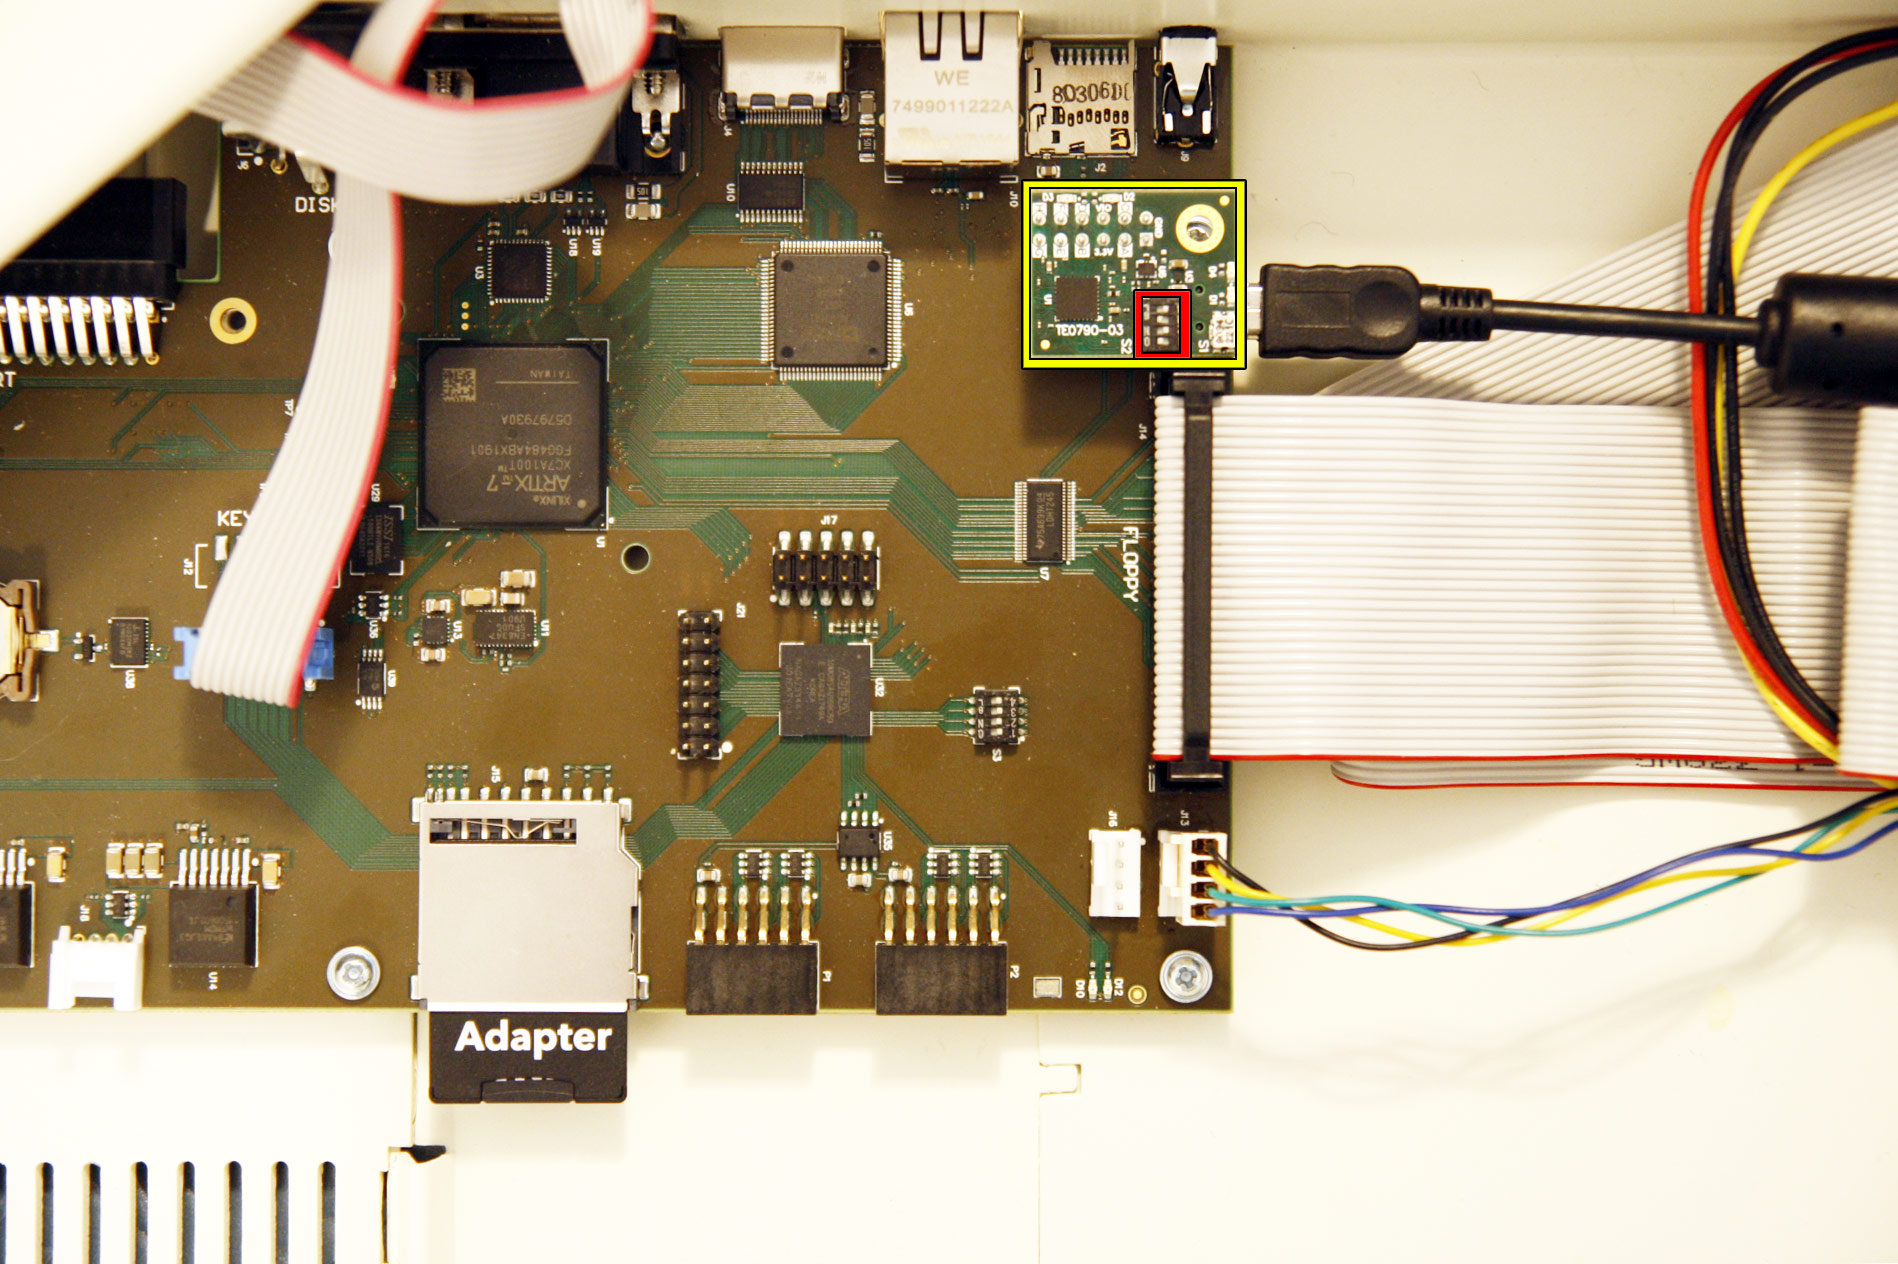
\includegraphics[width=\linewidth]{images/jtag_detail_02.jpg}

Connect your non-8-bit computer to the FPGA programming device using a
mini-USB cable. Switch the MEGA65 computer ON. Open VIVADO, which can
be downloaded from the Internet.

\newpage


\begin{figure}[H]
\centering
  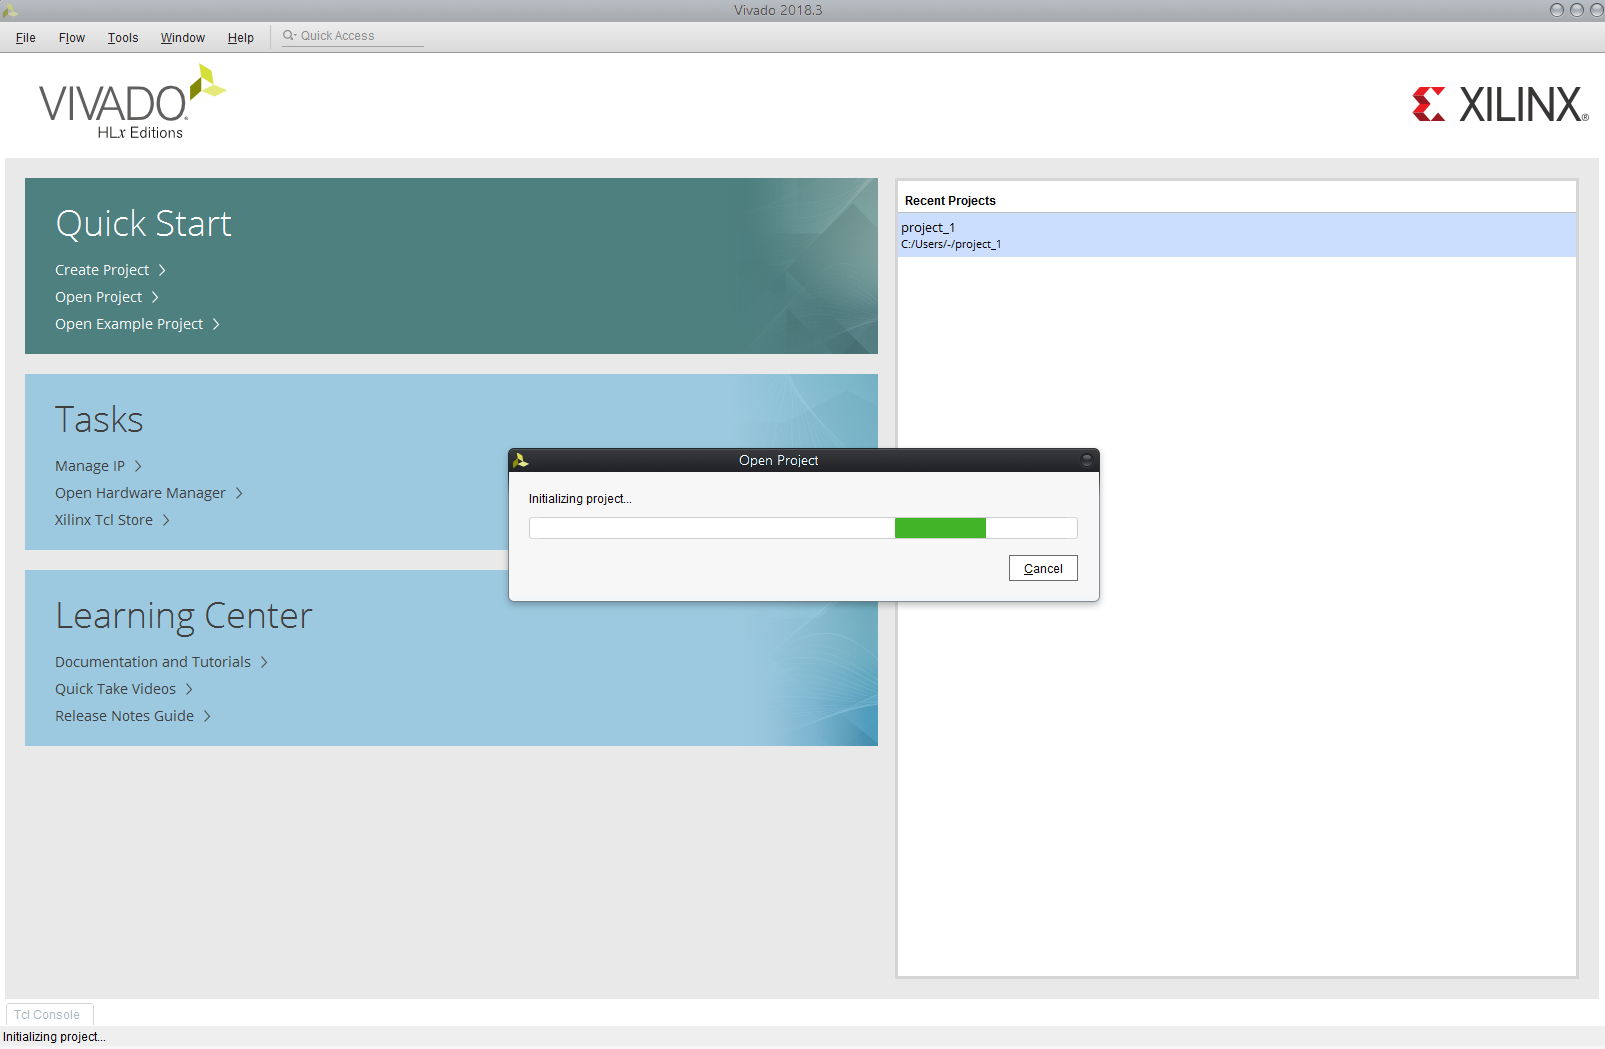
\includegraphics[width=0.8\linewidth]{images/vivado01.png}
  \captionsetup{width=0.8\linewidth}
  \caption{Step 1: To access the Hardware Manager, open a project in
           VIVADO or create an empty one, if you do not have any projects yet.}
  \label{fig:vivado01}
%\end{figure}

\vspace{5mm}

%\begin{figure}[H]
\centering
  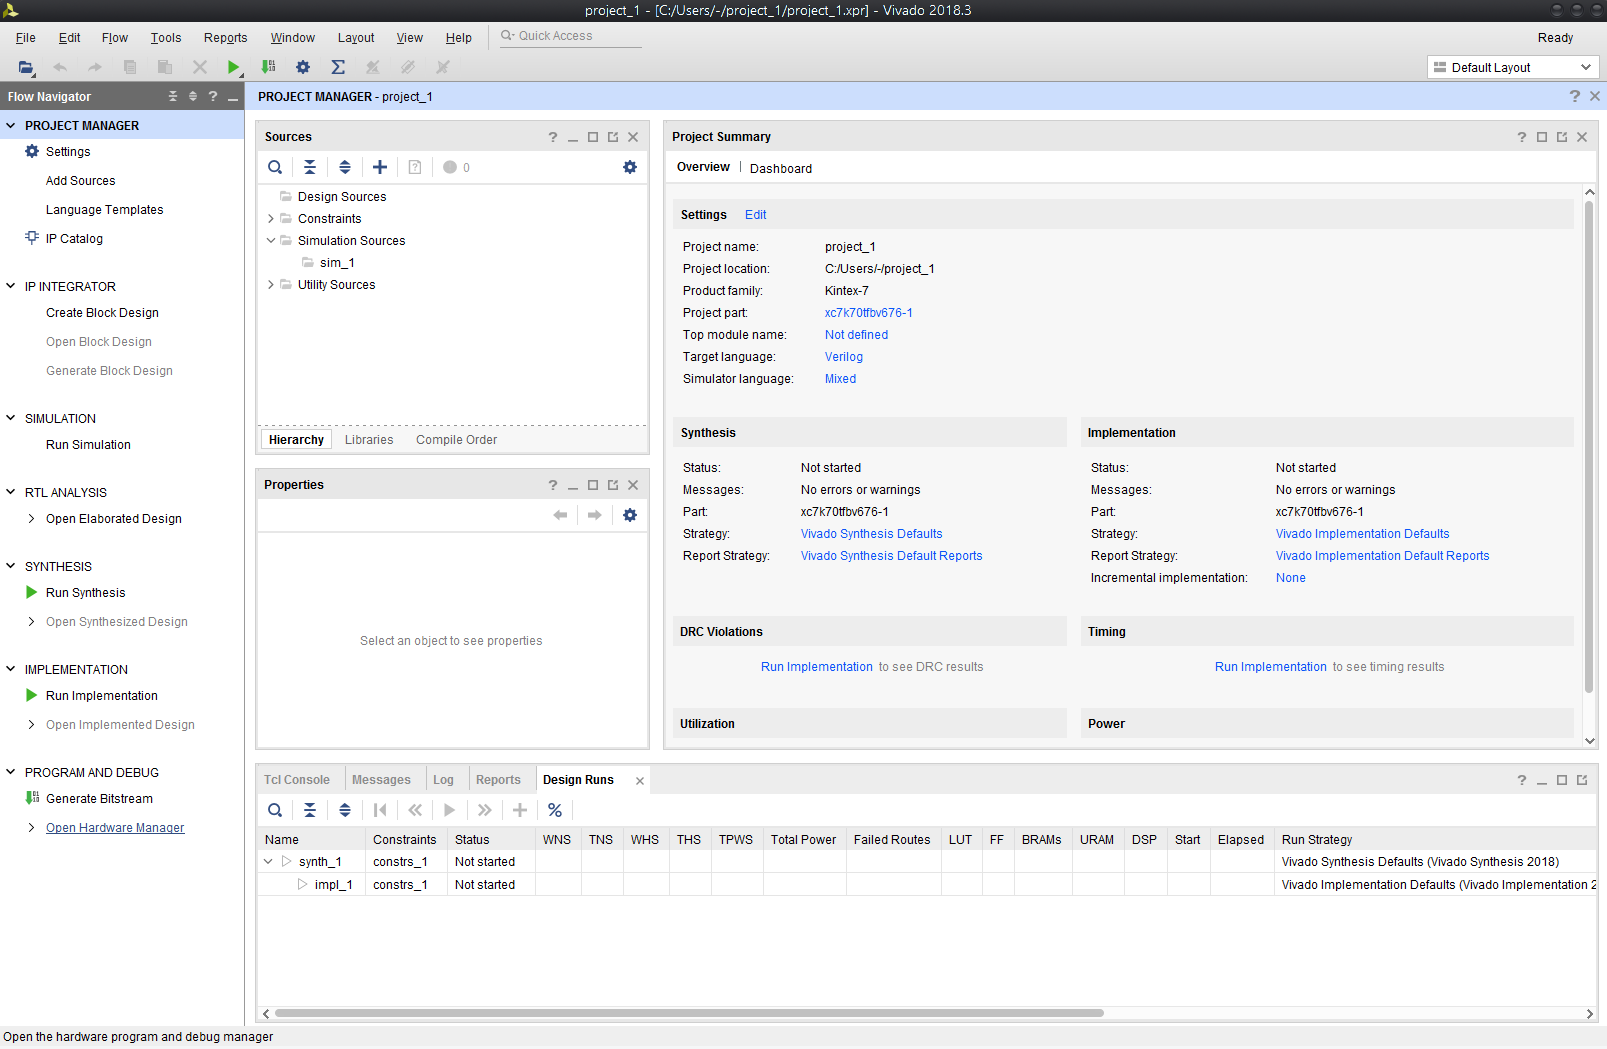
\includegraphics[width=0.8\linewidth]{images/vivado02.png}
  \captionsetup{width=0.8\linewidth}
  \caption{Step 2: In the left column, select "Open Hardware Manager"
           at the very bottom.}
  \label{fig:vivado02}
\end{figure}


\begin{figure}[H]
  \centering
  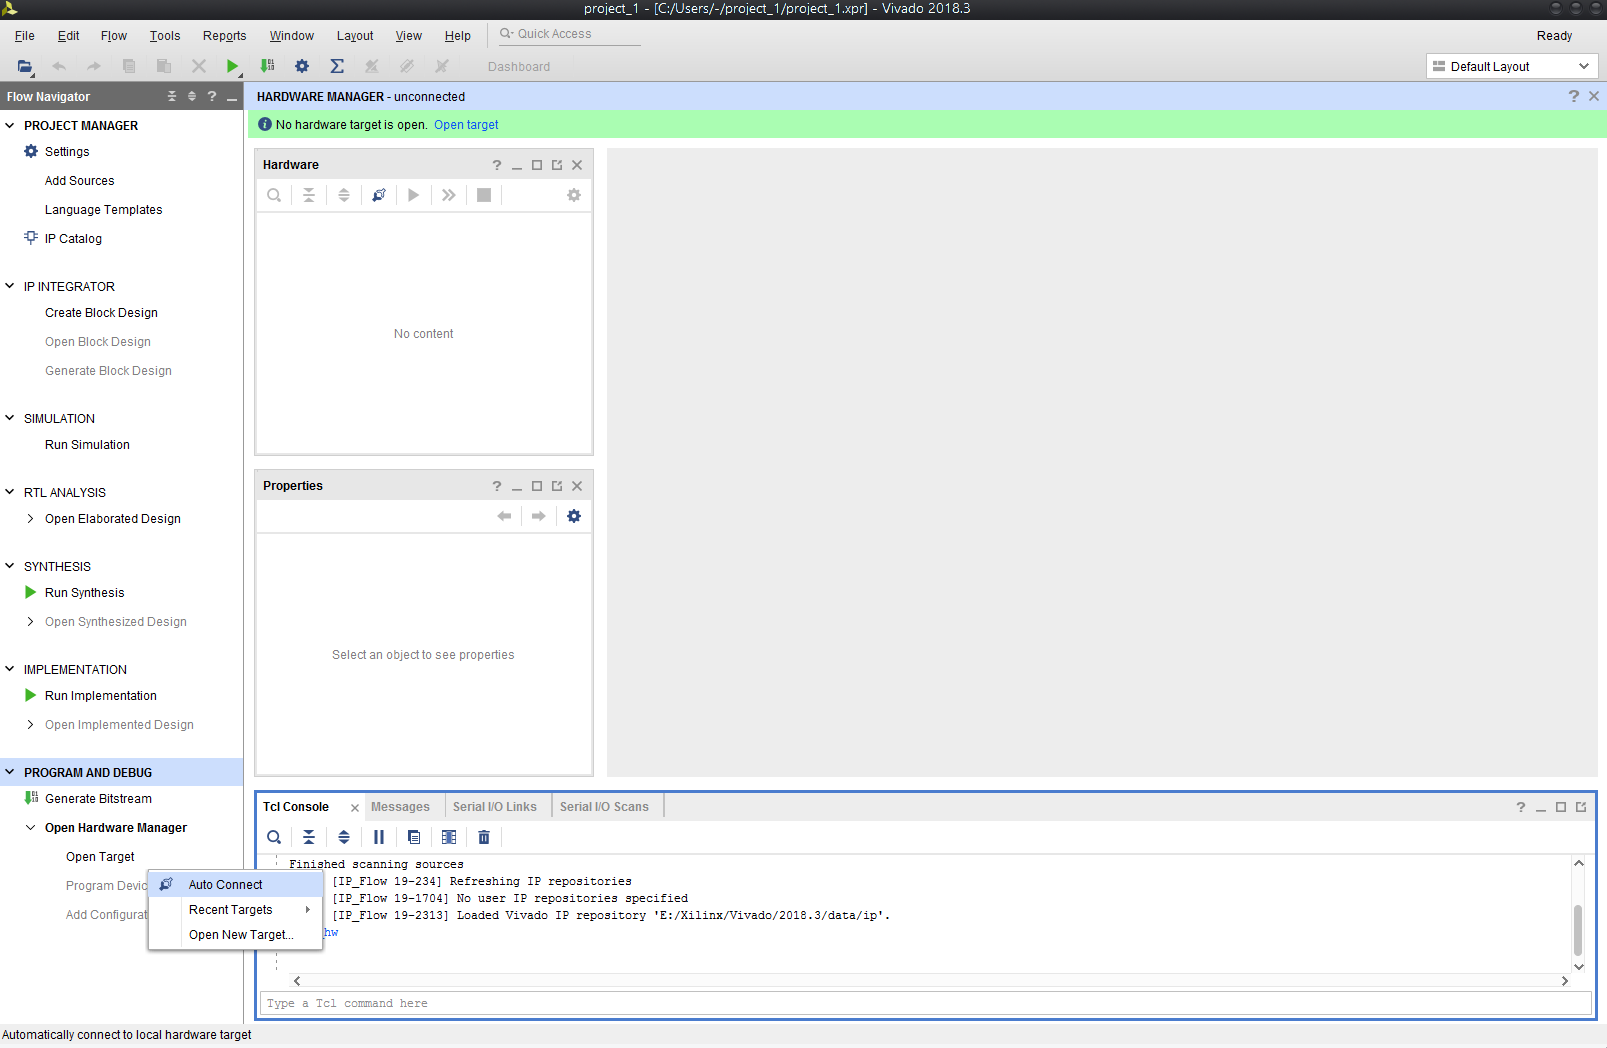
\includegraphics[width=0.8\linewidth]{images/vivado03.png}
  \captionsetup{width=0.8\linewidth}
  \caption{Step 3: To connect to FPGA
           under "Hardware Manager", choose "Open Target", then "Auto Connect".}
  \label{fig:vivado03}
%\end{figure}

\vspace{5mm}

%\begin{figure}[H]
  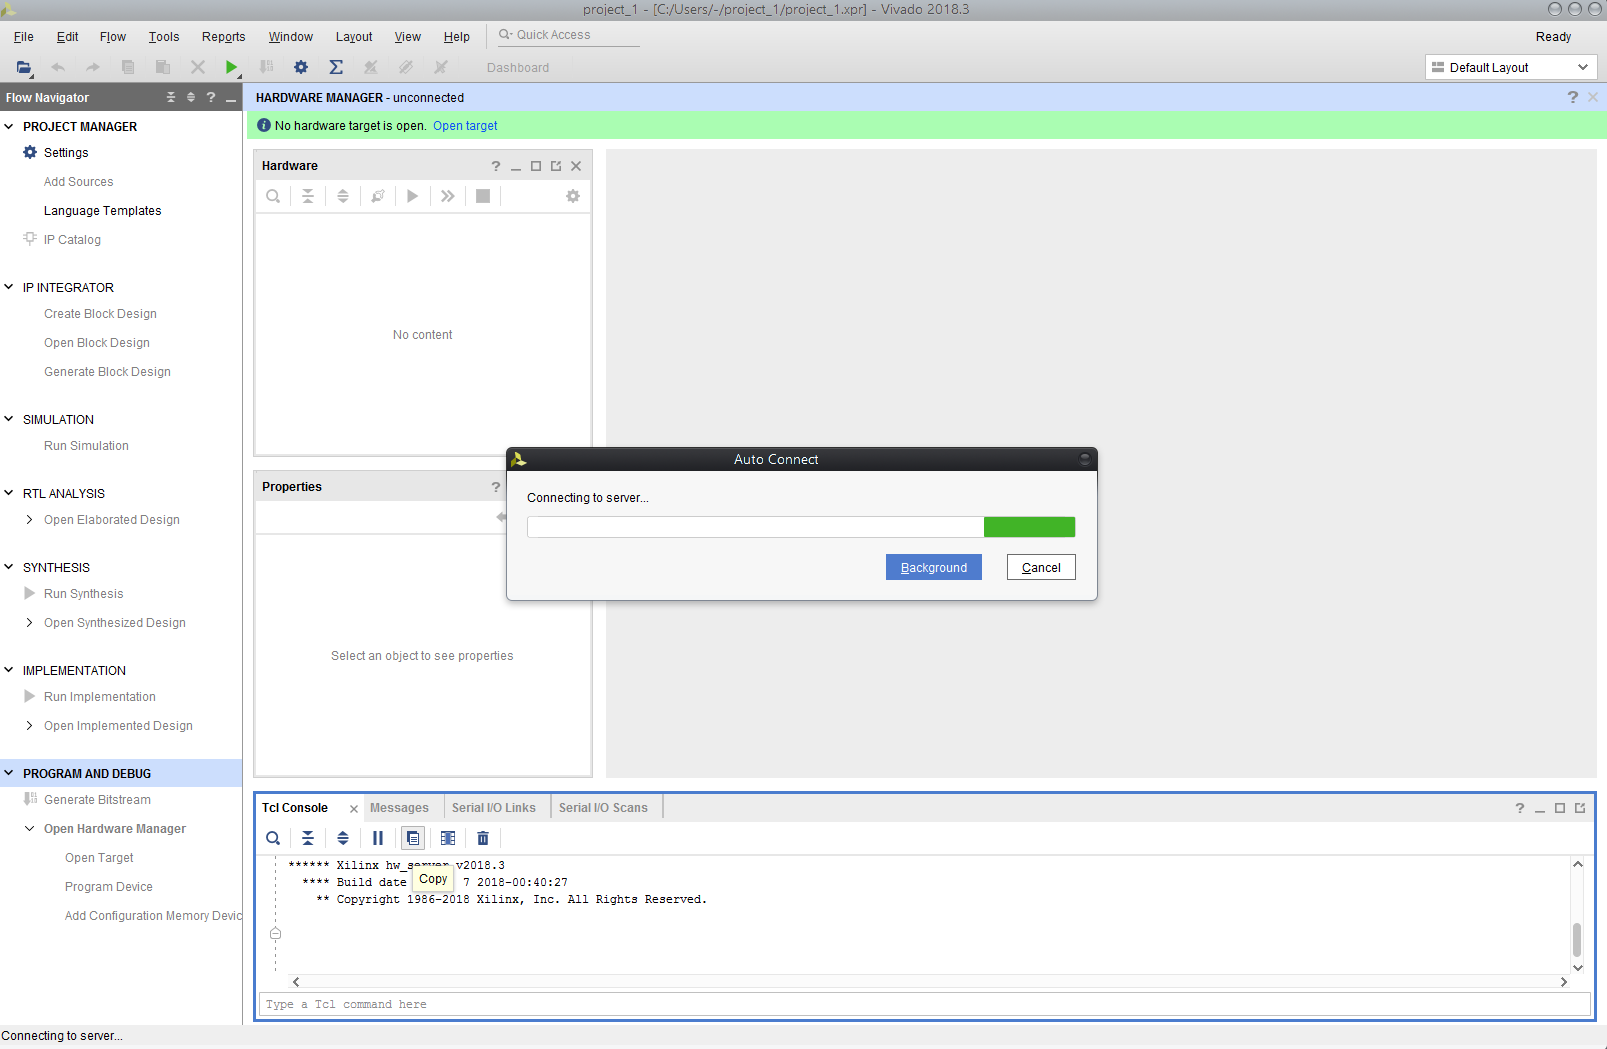
\includegraphics[width=0.8\linewidth]{images/vivado04.png}
  \captionsetup{width=0.8\linewidth}
  \caption{Step 4: Wait a moment, "Connecting to server..."  should
           automatically close without dropping an error to the console.}
  \label{fig:vivado04}
\end{figure}


\begin{figure}[H]
  \centering
  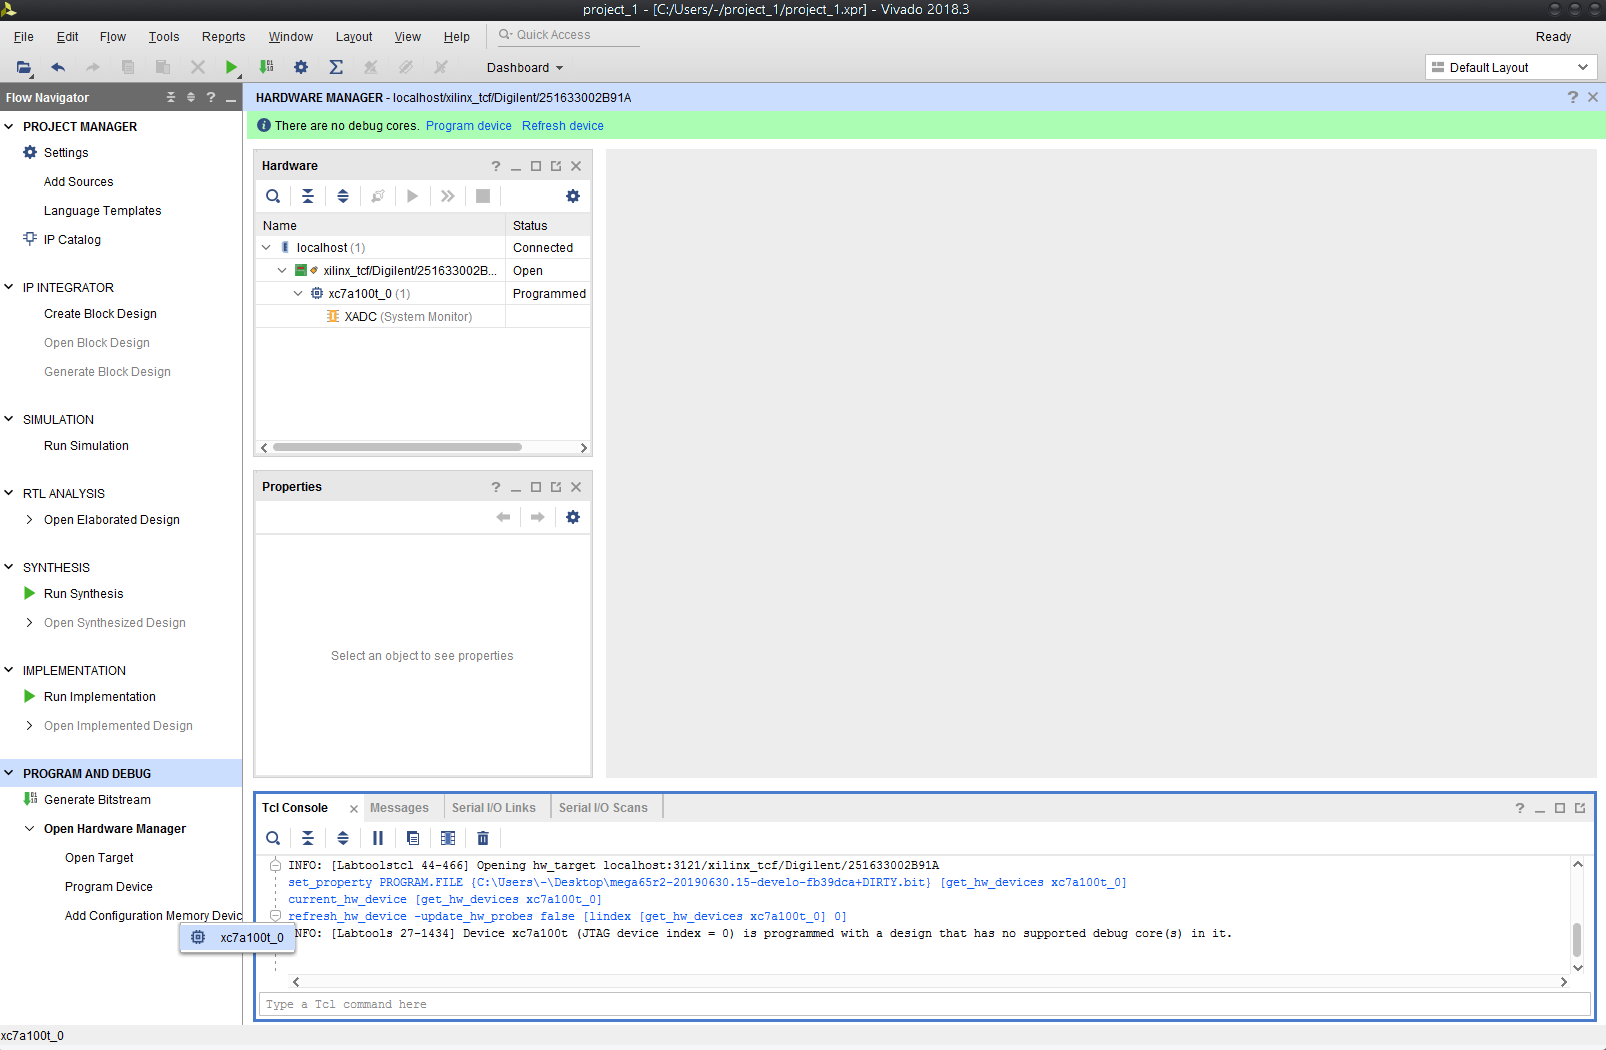
\includegraphics[width=0.8\linewidth]{images/vivado05.png}
  \captionsetup{width=0.8\linewidth}
  \caption{Step 5: Under "Hardware Manager", choose "Add Configuration
           Memory Device", then "xc7a100t\_0".}
  \label{fig:vivado05}
%\end{figure}

\vspace{5mm}

%\begin{figure}[H]
  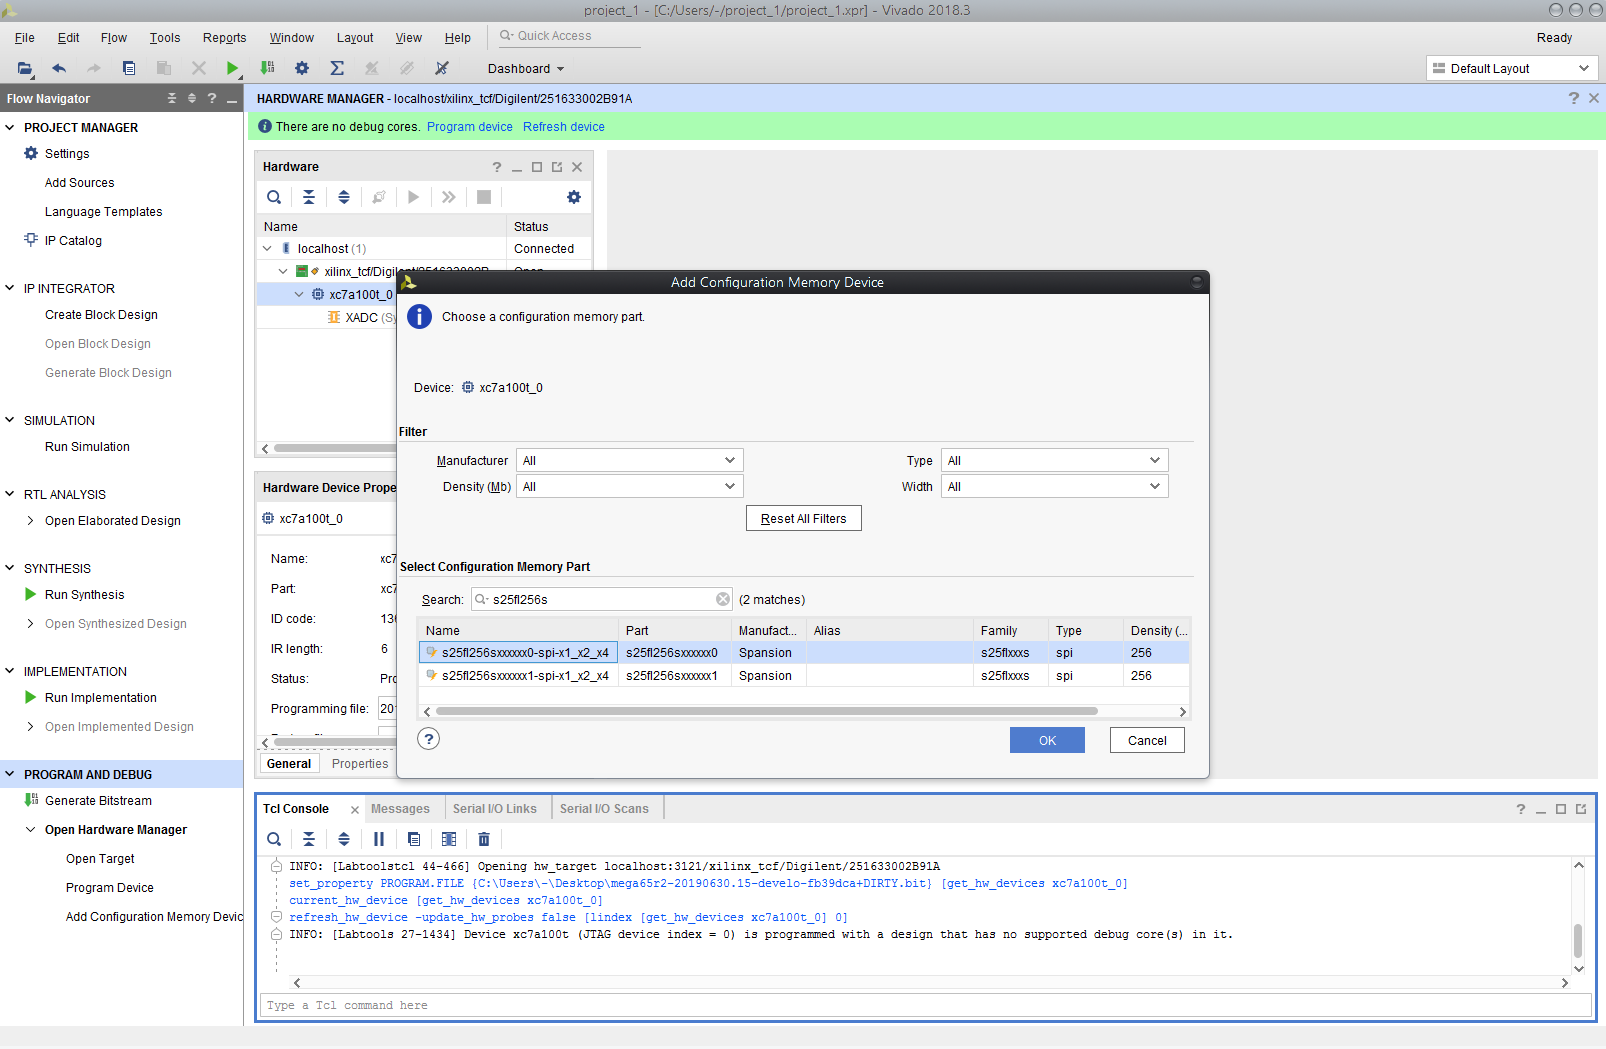
\includegraphics[width=0.8\linewidth]{images/vivado06.png}
  \captionsetup{width=0.8\linewidth}
  \caption{Step 6: Select Memory Part:
           In the newly opened dialogue, type "S25fl256s"
           (without quotes), then select "s25fl256sxxxxxxx0-spi-x1\_x2\_x4"
           (the upper one) and click "OK".}
  \label{fig:vivado06}
\end{figure}


\begin{figure}[H]
  \centering
  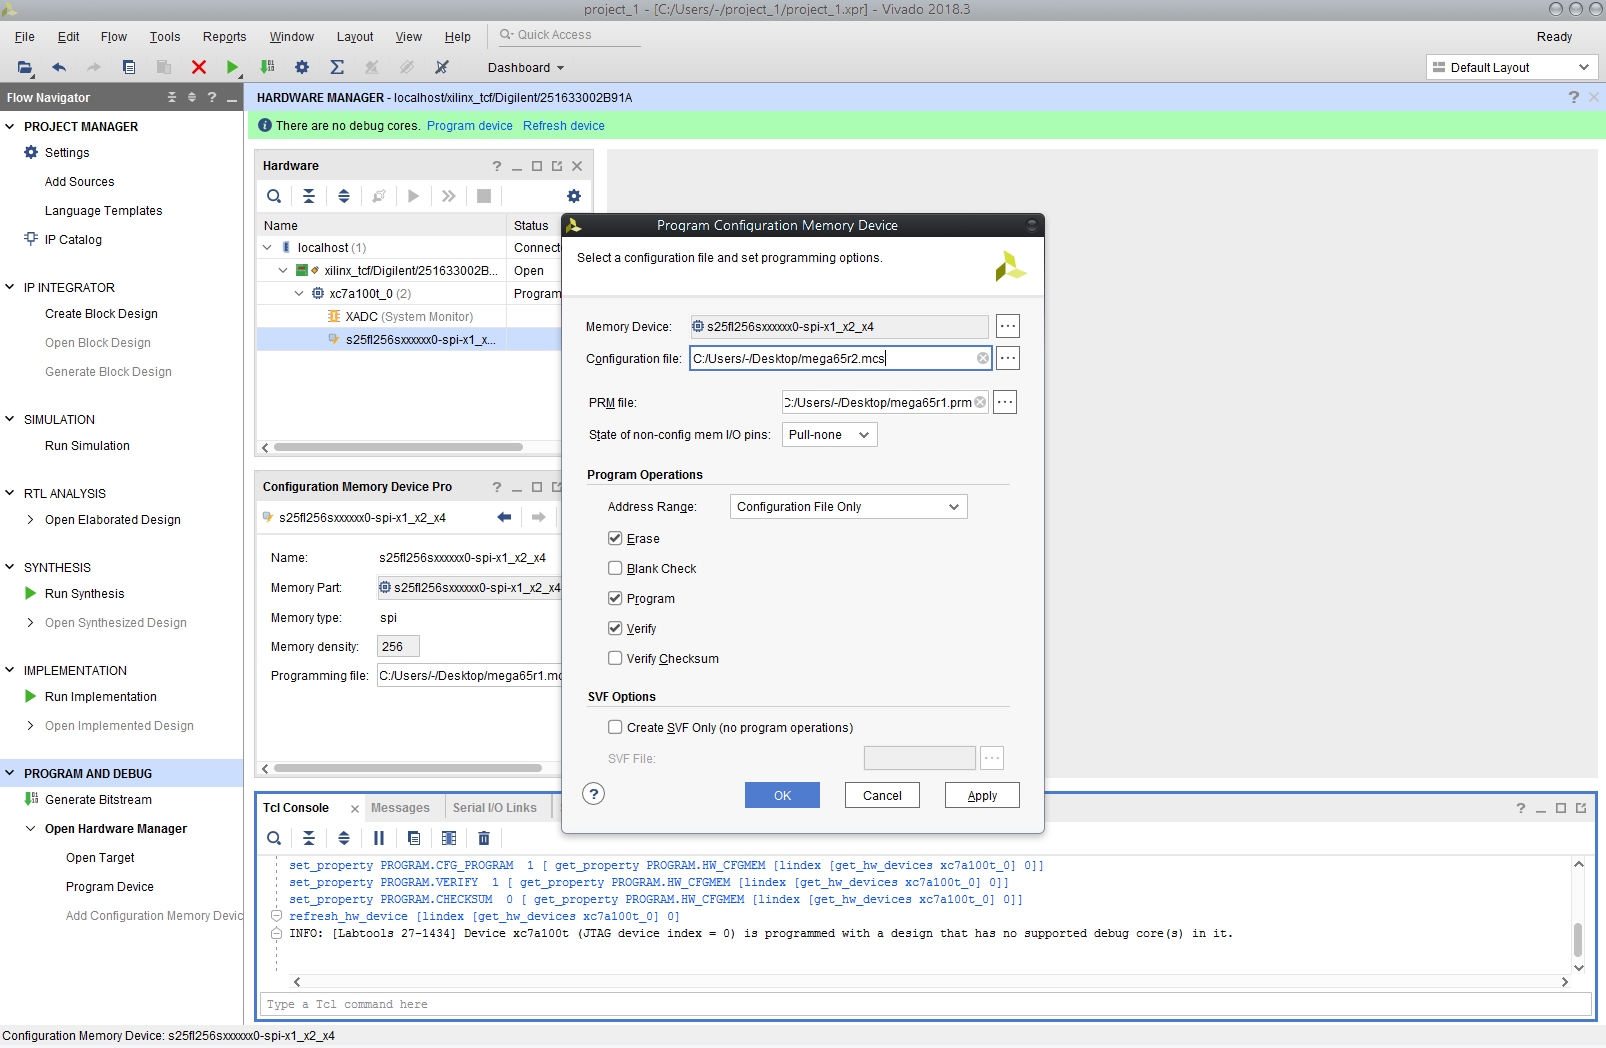
\includegraphics[width=0.85\linewidth]{images/vivado07.png}
  \captionsetup{width=0.85\linewidth}
  \caption{Step 7: Set programming options:
           In the next dialogue, choose your local Configuration file, namely
           a bitstream with file suffix ".mcs". Leave all other parameters
           as they are (see \ref{fig:vivado07}).}
  \label{fig:vivado07}
%\end{figure}

\vspace{3mm}

%\begin{figure}[H]
  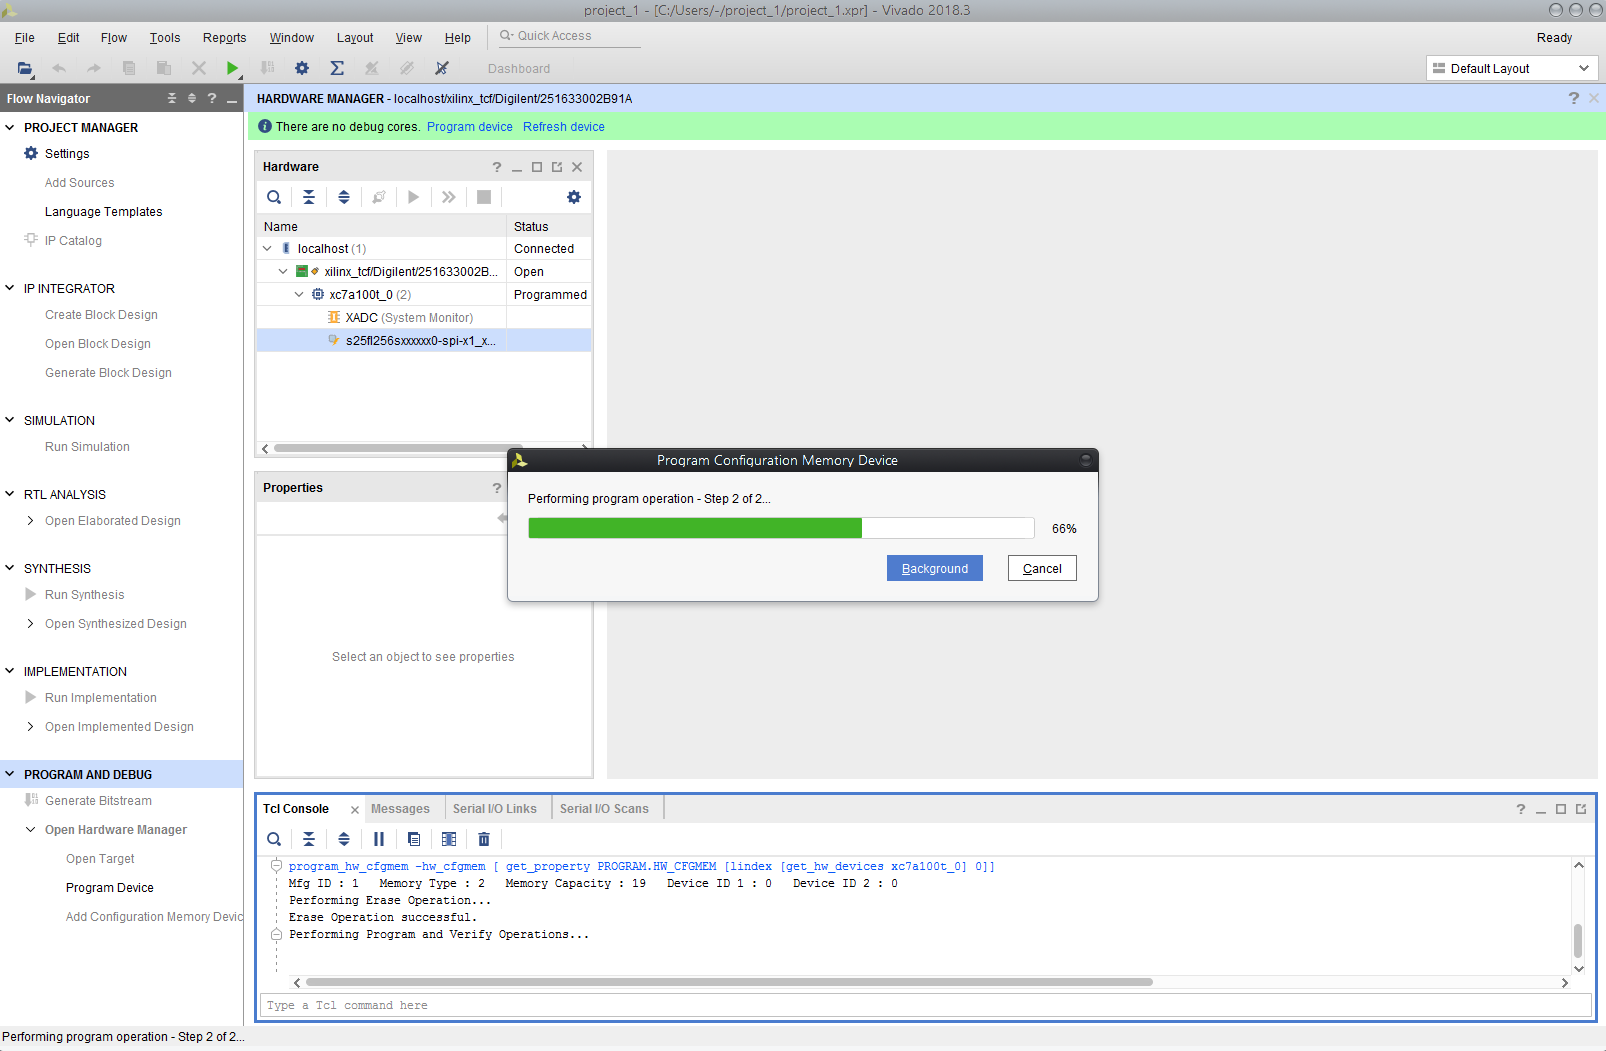
\includegraphics[width=0.85\linewidth]{images/vivado08.png}
  \captionsetup{width=0.85\linewidth}
  \caption{Step 8: Patiently wait for the programming to finish.
           This can take several minutes as the Vivado software erases
           and then reprograms the flash memory that is used to
           initialise the FPGA on power-up.}
  \label{fig:vivado08}
\end{figure}


\begin{figure}[H]
  \centering
  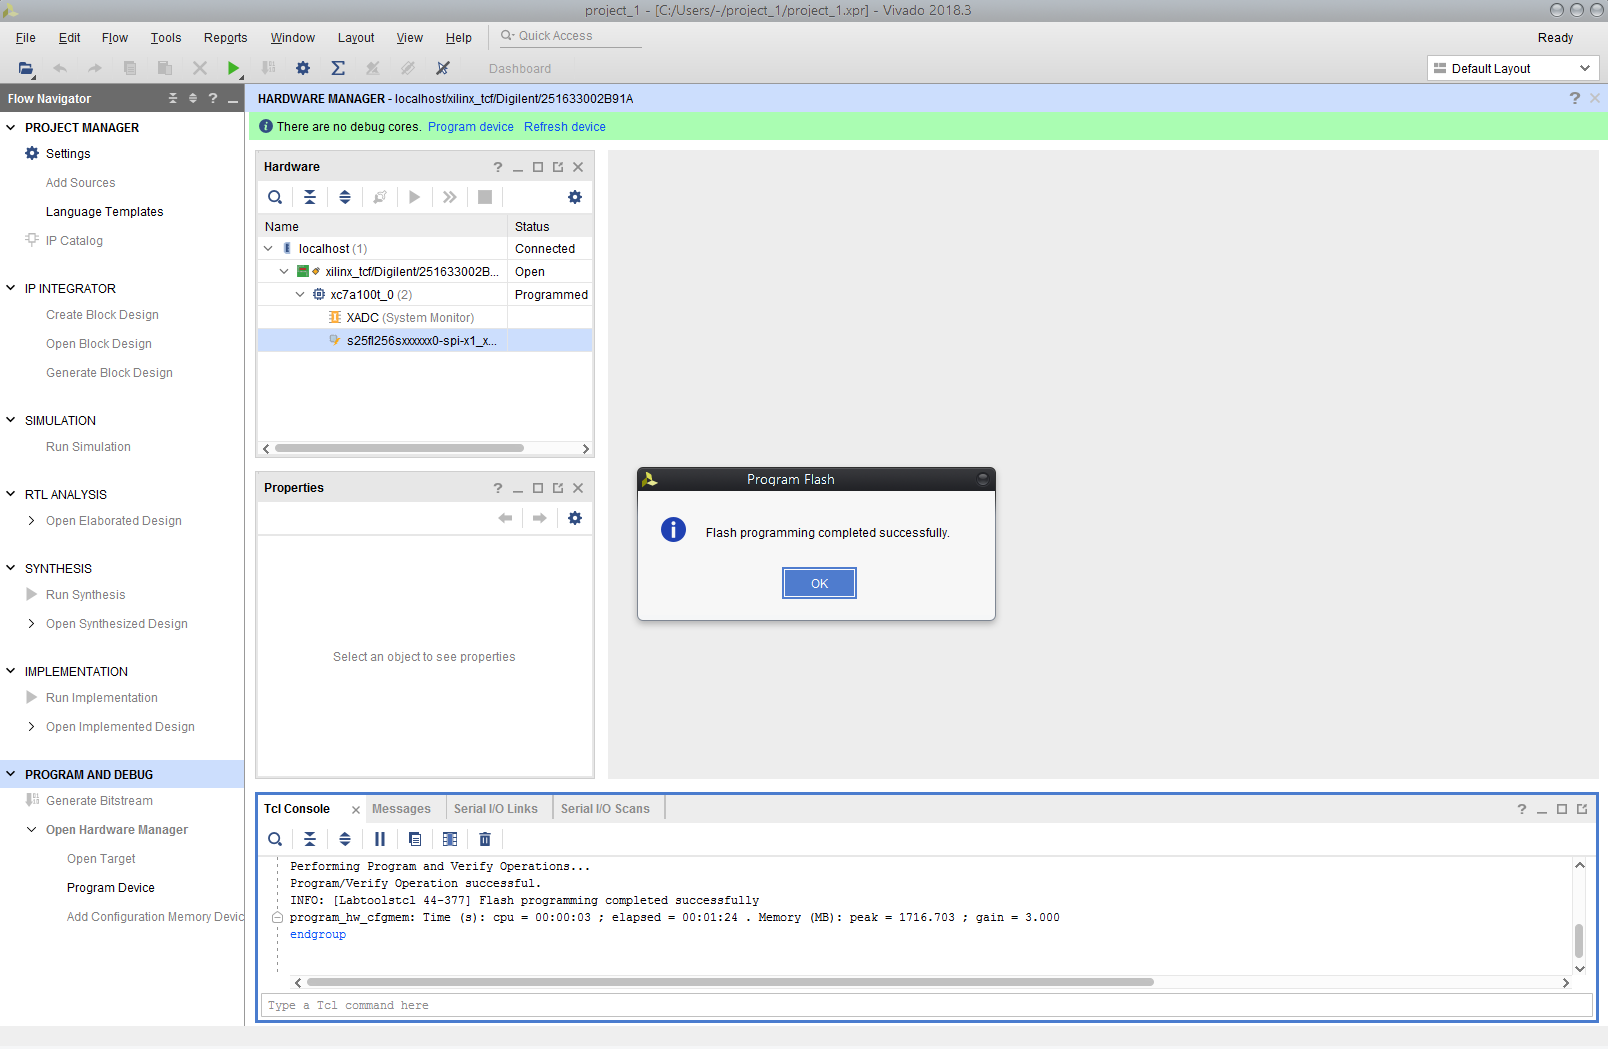
\includegraphics[width=0.8\linewidth]{images/vivado09.png}
  \captionsetup{width=0.8\linewidth}
  \caption{Step 9: If your screen looks like \ref{fig:vivado09},
           your new bistream has been successfully flashed into the Artix 100T FPGA!}
  \label{fig:vivado09}
%\end{figure}

\vspace{5mm}

%\begin{figure}[H]
  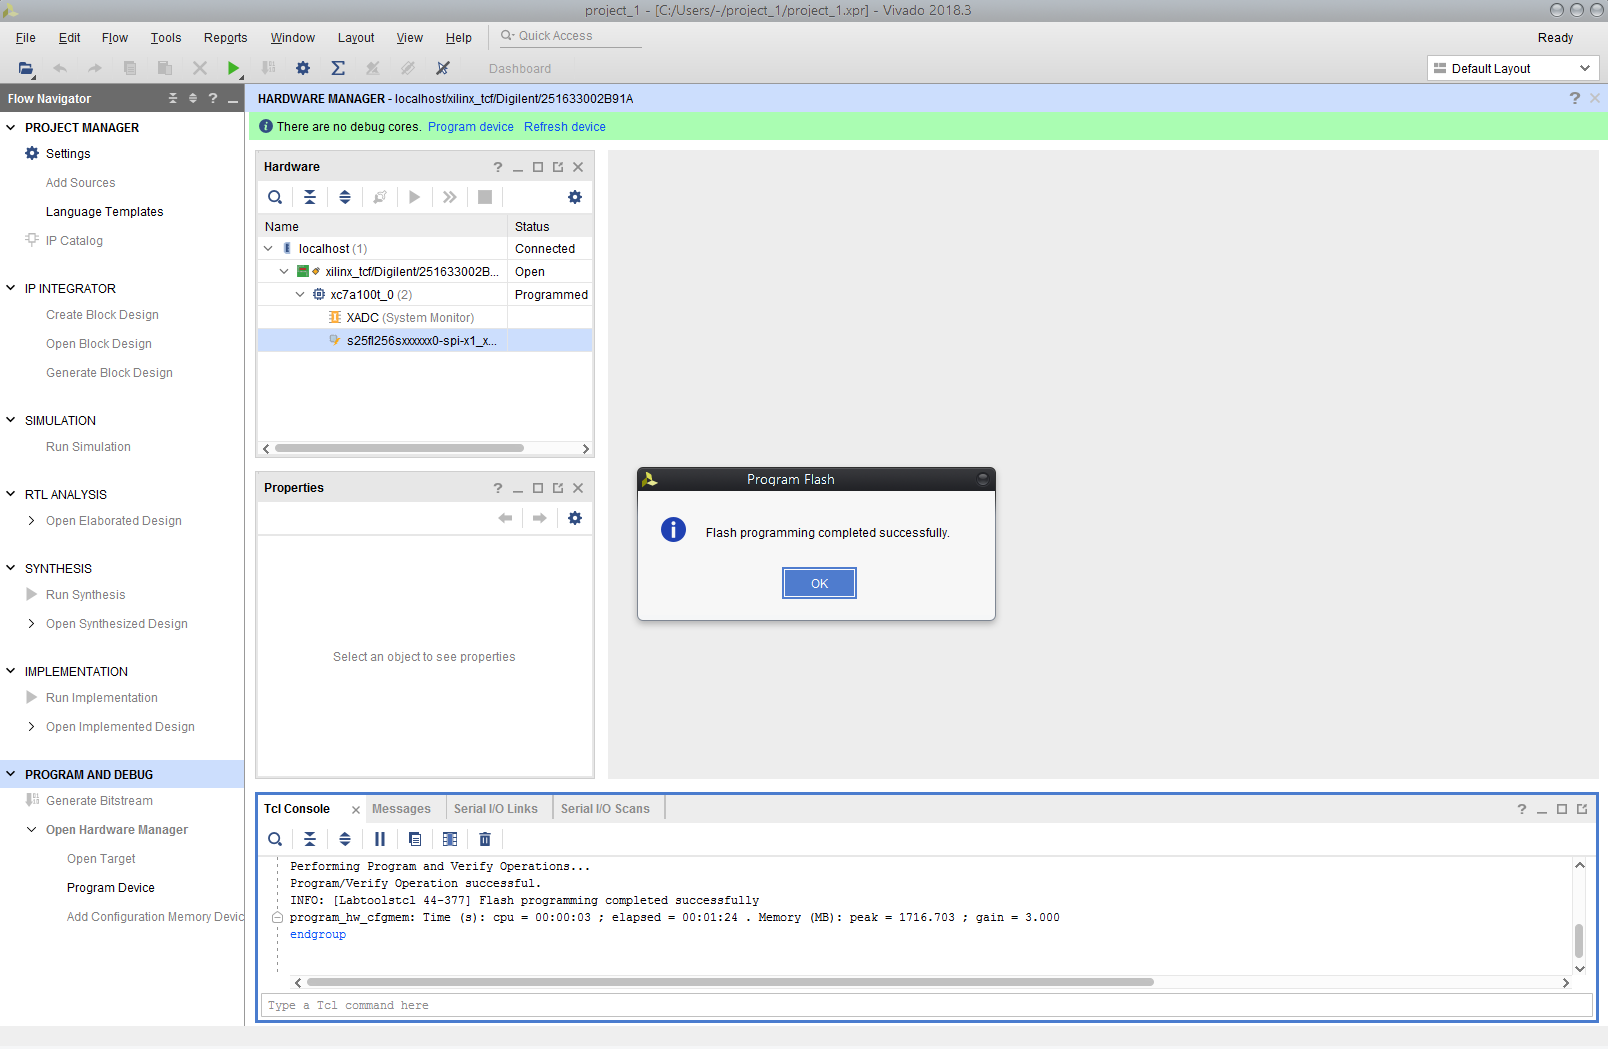
\includegraphics[width=0.8\linewidth]{images/vivado09.png}
  \captionsetup{width=0.8\linewidth}
  \caption{Step 10: If you want to reflash the FPGA, you might find the
  "Add Configuration Memory Device" option in step 5 greyed out.
   Instead, select "s25fl256sxxxxxxx0-spi-x1\_x2\_x4"  in the "Hardware"
   window, press right mouse button and select "Program Configuration
   Memory Device" to flash.}
  \label{fig:vivado10}
\end{figure}


\section{Flashing the CPLD in the MEGA65's Keyboard with LATTICE DIAMOND}


If you choose to proceed, you will need a TE0790-03 JTAG programming
module, a functioning installation of Lattice Diamond Programmer software.
This can be done on either Windows or Linux, but in both cases you will
need to install any necessary USB drivers. It is also necessary to have
dip-switches 1 and 3 in the ON position and dip-switches 2 and 4 in the
OFF position on the TE-0790. With your MEGA65 disconnected from the power,
the TE-0790 must be installed on the JB1 connector, which is located
between the floppy data cable and the audio jack.
The gold-plated hole of the TE-0790 must line up with the screw hole below.
The mini-USB cable will then connect on the side towards the 3.5" floppy drive.
The following image shows the correct position: The TE0790 is surrounded
by the yellow box, and the dip-switches by the red box. Dip-switch 1 is
the one nearest the floppy data cable.


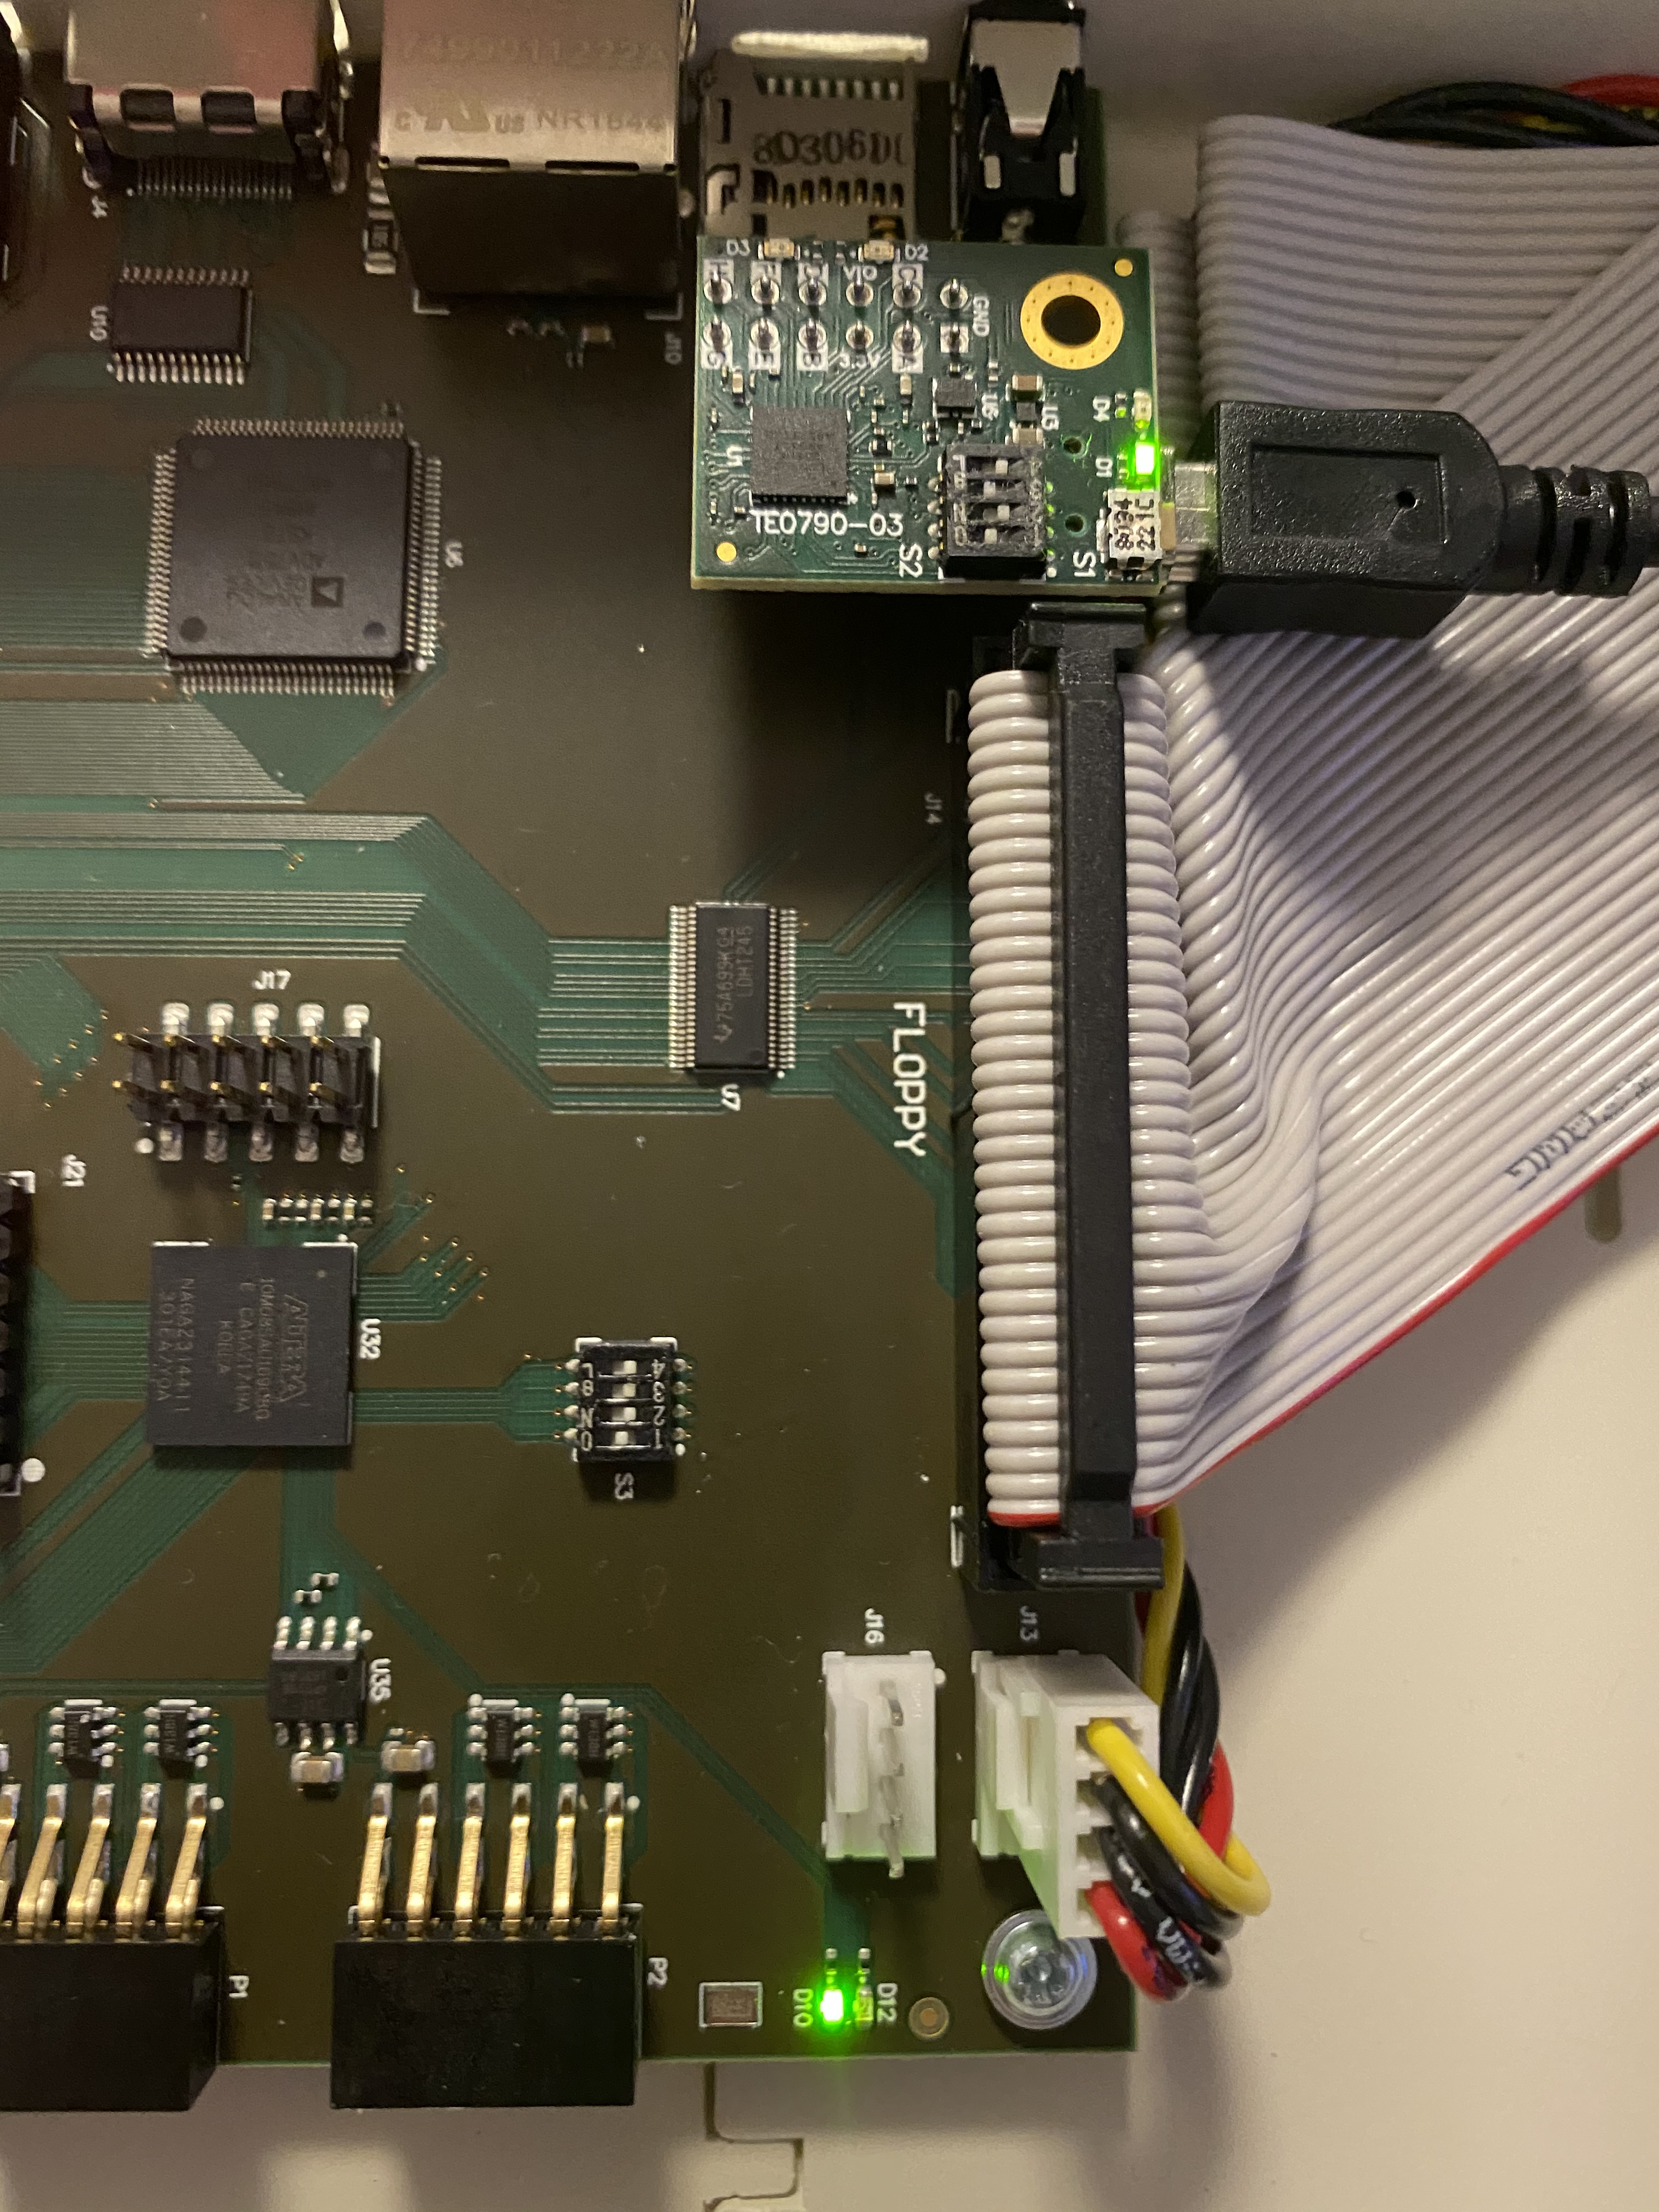
\includegraphics[width=\linewidth]{images/jtag_detail_05.jpg}


One the PCB r2 MEGA65 Mainboard dip switch 1 (the one nearest to the user
sitting in front of the machine must be in the ON position, the other
switches must be OFF. The keyboard will go into "Police Mode"
(blue and red blinking LEDs) when set correctly.

Connect your non-8-bit computer to the FPGA programming device using a
mini-USB cable. Switch the MEGA65 computer ON. Open DIAMOND PROGRAMMER,
which can be downloaded from the Internet.

\begin{figure}[H]
  \centering
  
\includegraphics{images/diamond01.png}
  \captionsetup{width=0.8\linewidth}
  \caption{Step 1: Open DIAMOND PROGRAMMER:
           Select "Create a new project from a JTAG scan". If entry
           under "Cable:" is empty, click "Detect Cable".}
  \label{fig:diamond01}
%\end{figure}

\vspace{5mm}

%\begin{figure}[H]
  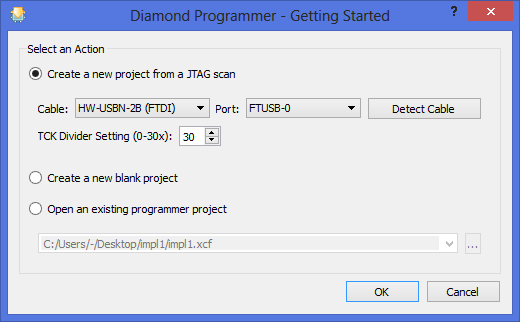
\includegraphics[width=0.8\linewidth]{images/diamond02.png}
  \captionsetup{width=0.8\linewidth}
  \caption{Step 2: Create a new project:
           If dialog "Programmer: Multiple Cables Detected" appears,
           select the first entry ("Location 0000") and click "OK".}
  \label{fig:diamond02}
\end{figure}


\begin{figure}[H]
  \centering
  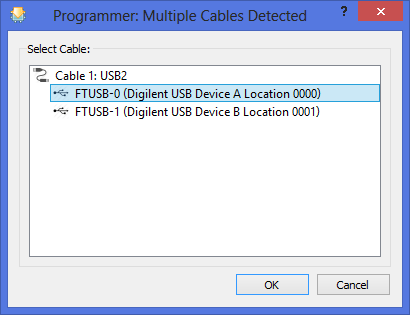
\includegraphics[width=0.8\linewidth]{images/diamond03.png}
  \captionsetup{width=0.8\linewidth}
  \caption{Step 3: Select cable:
           You have now created a new project which should display
           "MachXO2" under "Device Family" and "LCMXO2-1200HC" under "Device"}
  \label{fig:diamond03}
%\end{figure}

\vspace{5mm}

%\begin{figure}[H]
  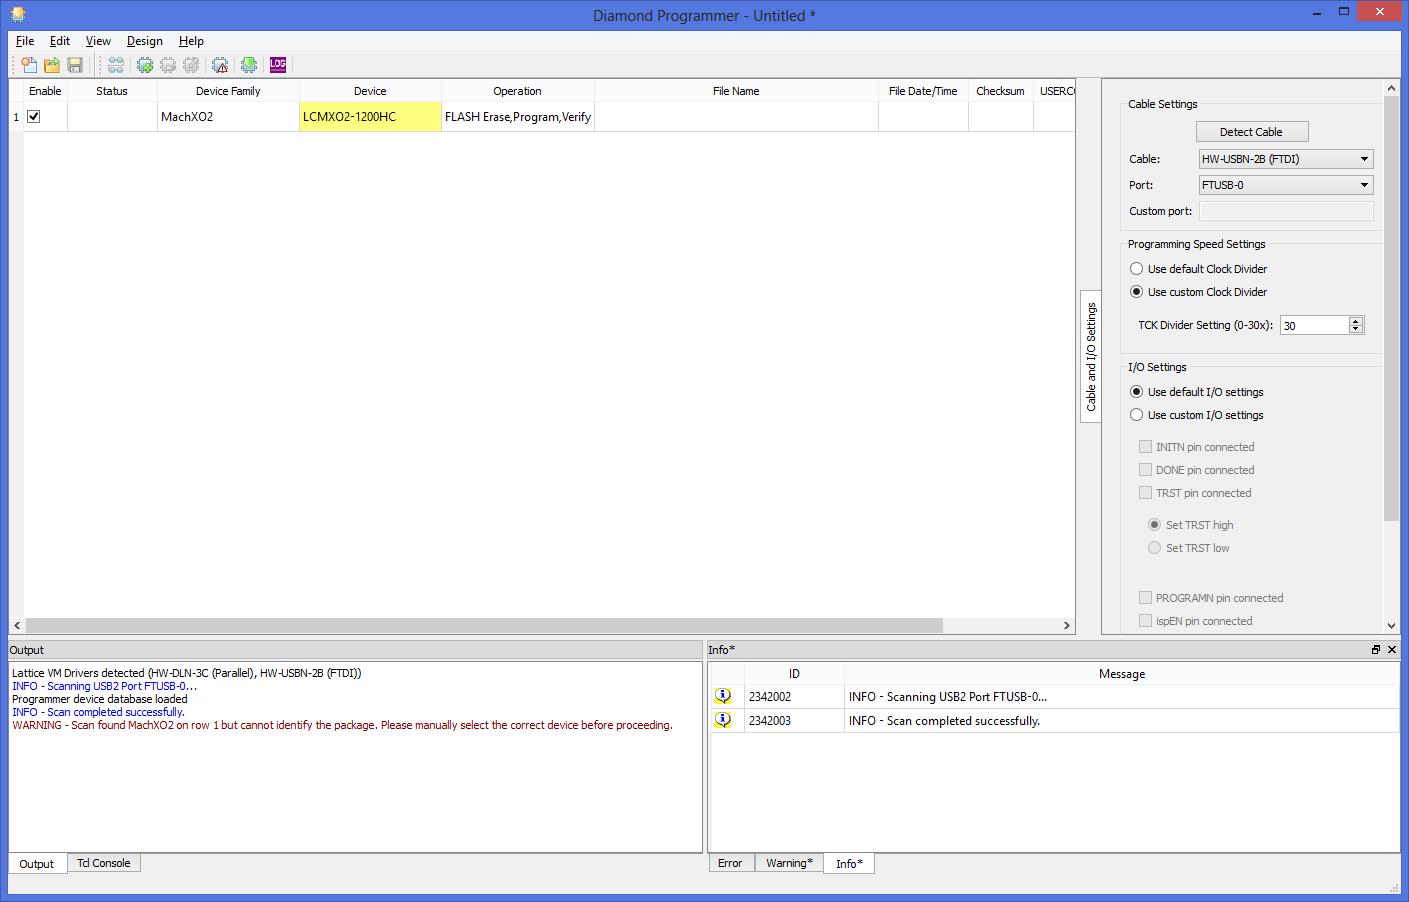
\includegraphics[width=0.8\linewidth]{images/diamond04.png}
  \captionsetup{width=0.8\linewidth}
  \caption{Step 4: New Diamond Programmer project:
           Choose "File"  then "Open File" to load the DIAMOND PROGRAMMER
           project with the MEGA65 keyboard firmware update.}
  \label{fig:diamond04}
\end{figure}


\begin{figure}[H]
  \centering
  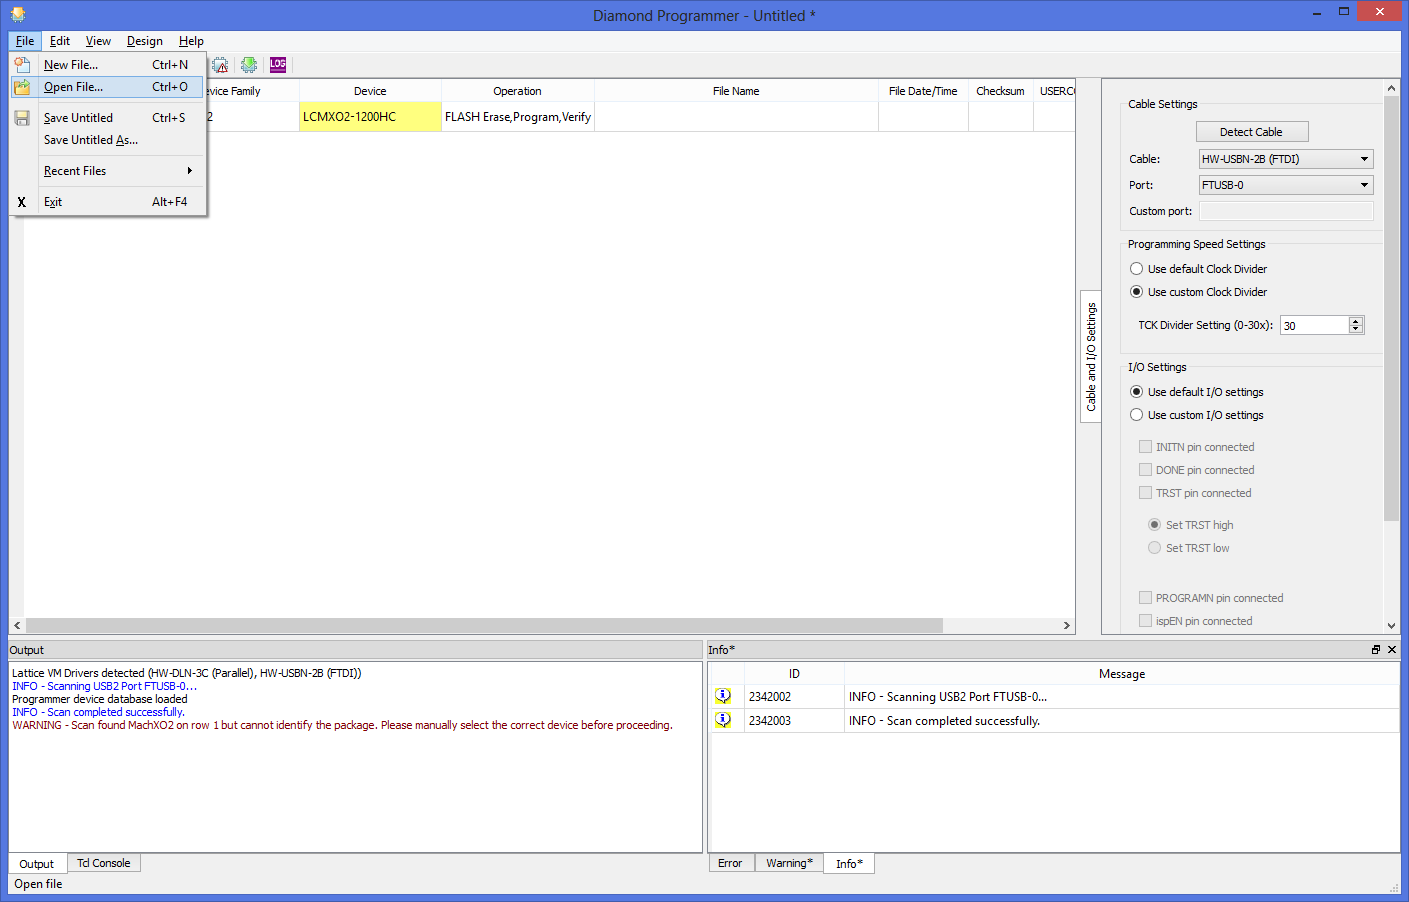
\includegraphics[width=0.8\linewidth]{images/diamond05.png}
  \captionsetup{width=0.8\linewidth}
  \caption{Step 5: Open project:
           Navigate into the folder with the extracted MEGA65 keyboard
           firmware files you have received and select the file ending with ".xcf".}
  \label{fig:diamond05}
%\end{figure}

\vspace{5mm}

%\begin{figure}[H]
  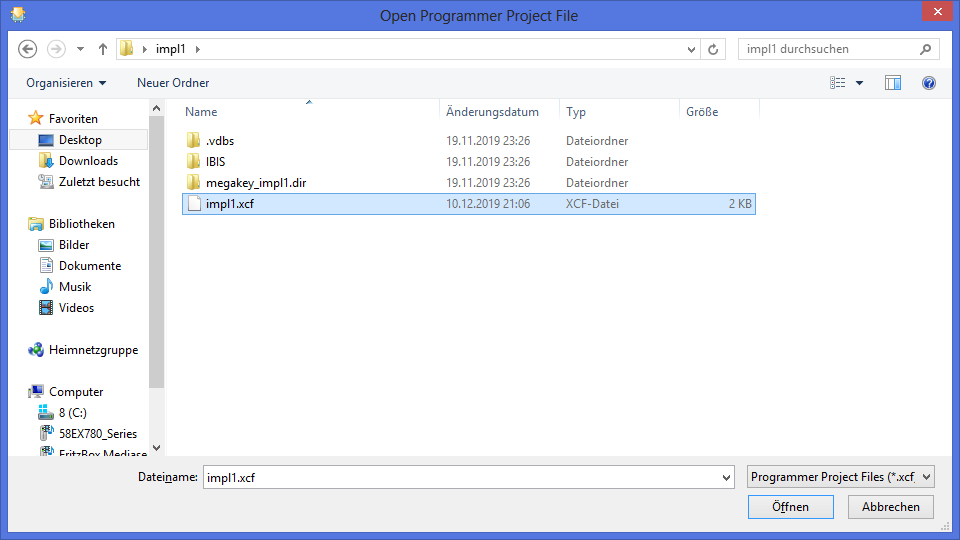
\includegraphics[width=0.8\linewidth]{images/diamond06.png}
  \captionsetup{width=0.8\linewidth}
  \caption{Step 6: Select project file:
           Click the three dots under "File Name" to set the correct
           path and find the file ending with ".jed".}
  \label{fig:diamond06}
\end{figure}


\begin{figure}[H]
  \centering
  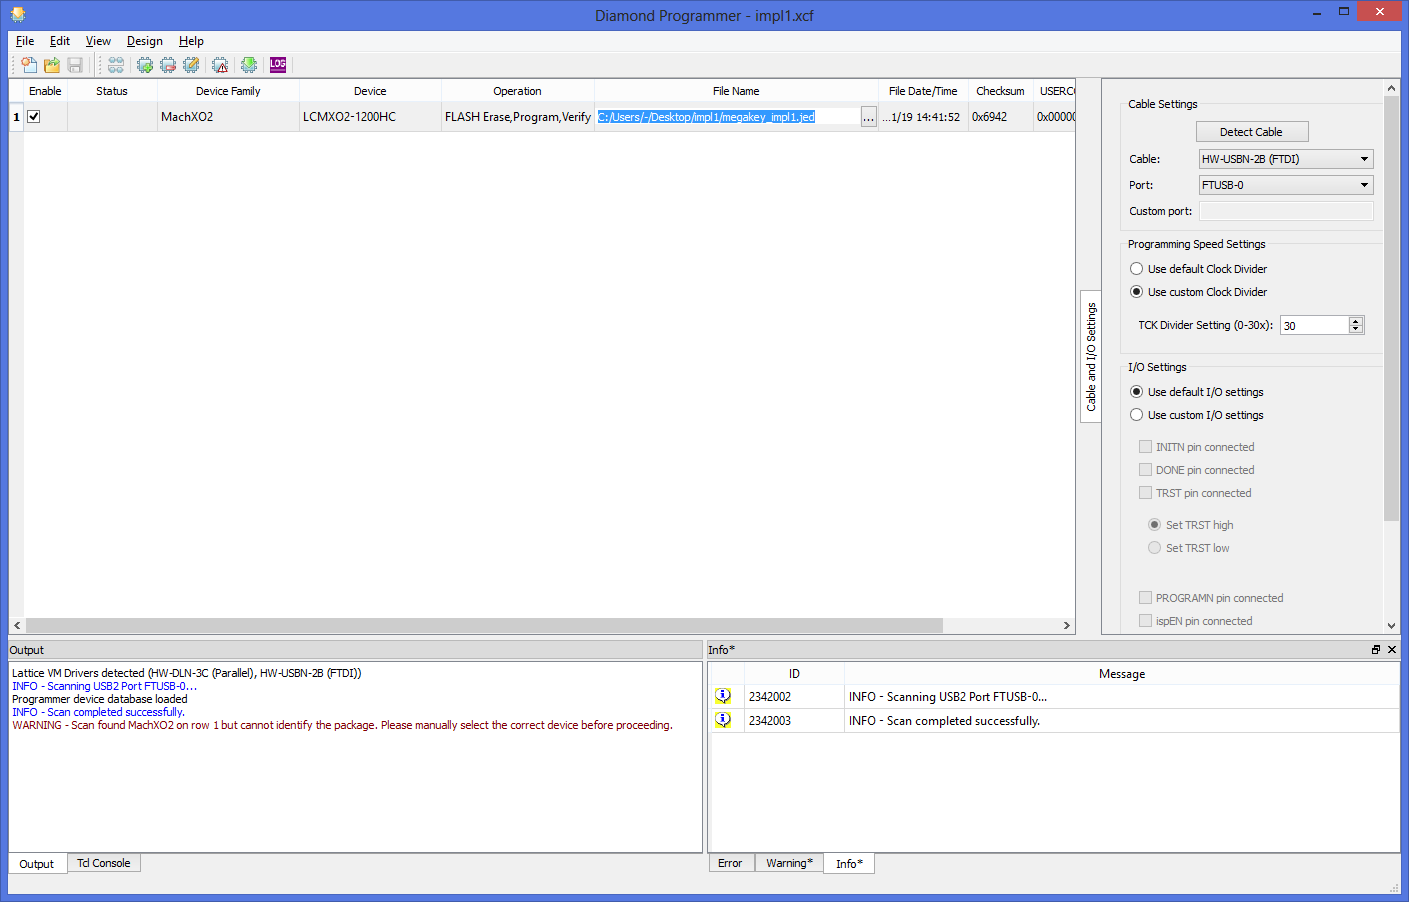
\includegraphics[width=0.8\linewidth]{images/diamond07.png}
  \captionsetup{width=0.8\linewidth}
  \caption{Step 7: Choose correct path of .jed file:
           Select the file ending with ".jed" and click "OK".}
  \label{fig:diamond07}
%\end{figure}

\vspace{5mm}

%\begin{figure}[H]
  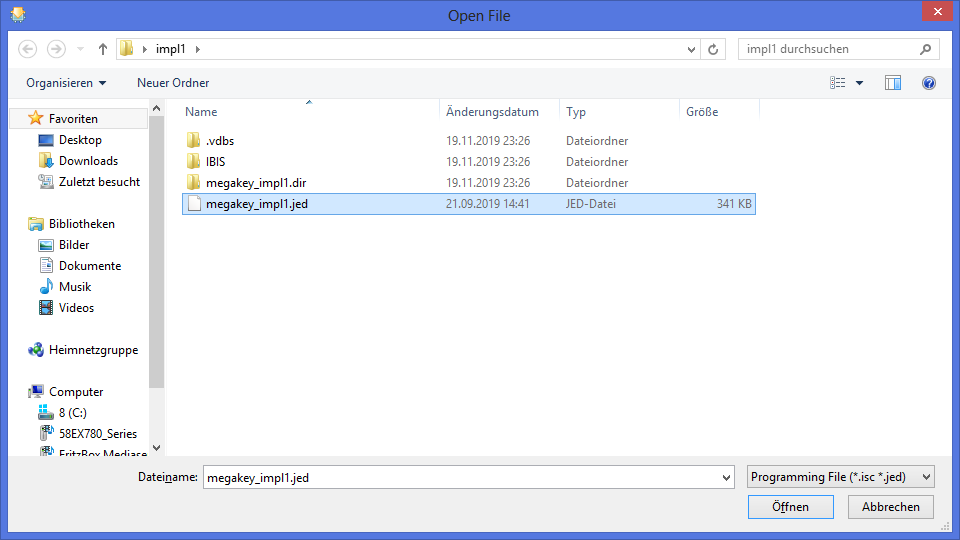
\includegraphics[width=0.8\linewidth]{images/diamond08.png}
  \captionsetup{width=0.8\linewidth}
  \caption{Step 8: Select .jed file:
           Click on the icon with the green arrow facing down "PROGRAM",
           which looks similar to the DIAMOND PROGRAMMER program icon.}
  \label{fig:diamond08}
\end{figure}


\begin{figure}[H]
  \centering
  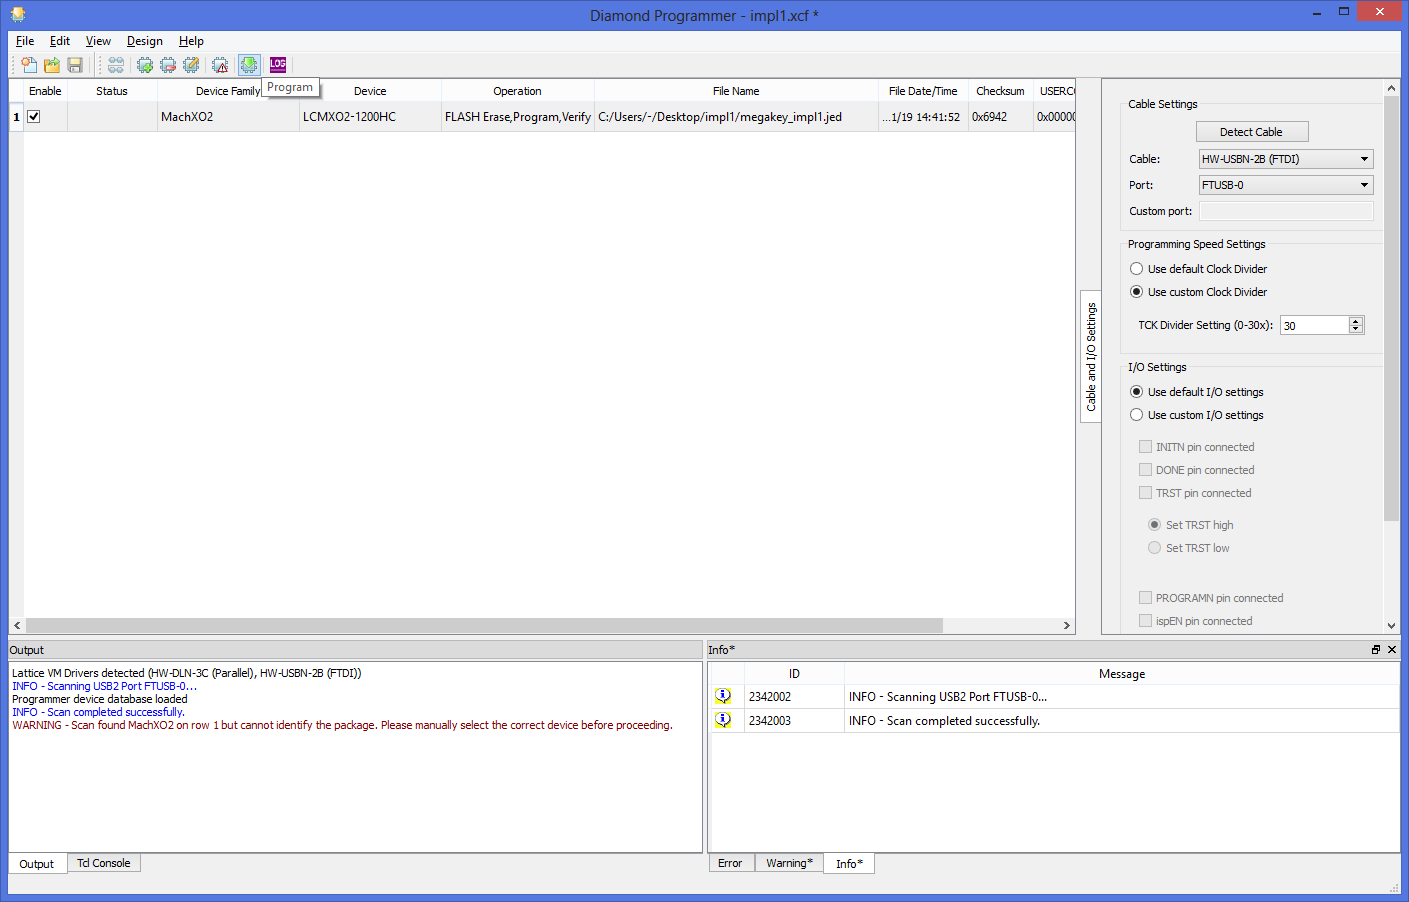
\includegraphics[width=0.8\linewidth]{images/diamond09.png}
  \captionsetup{width=0.8\linewidth}
  \caption{Step 9: Select cable:
           After a moment  the Output window should display
           "INFO - Operation: successful." and the "Status" cell should
           go green (does not always happen).}
  \label{fig:diamond09}
%\end{figure}

\vspace{5mm}

%\begin{figure}[H]
  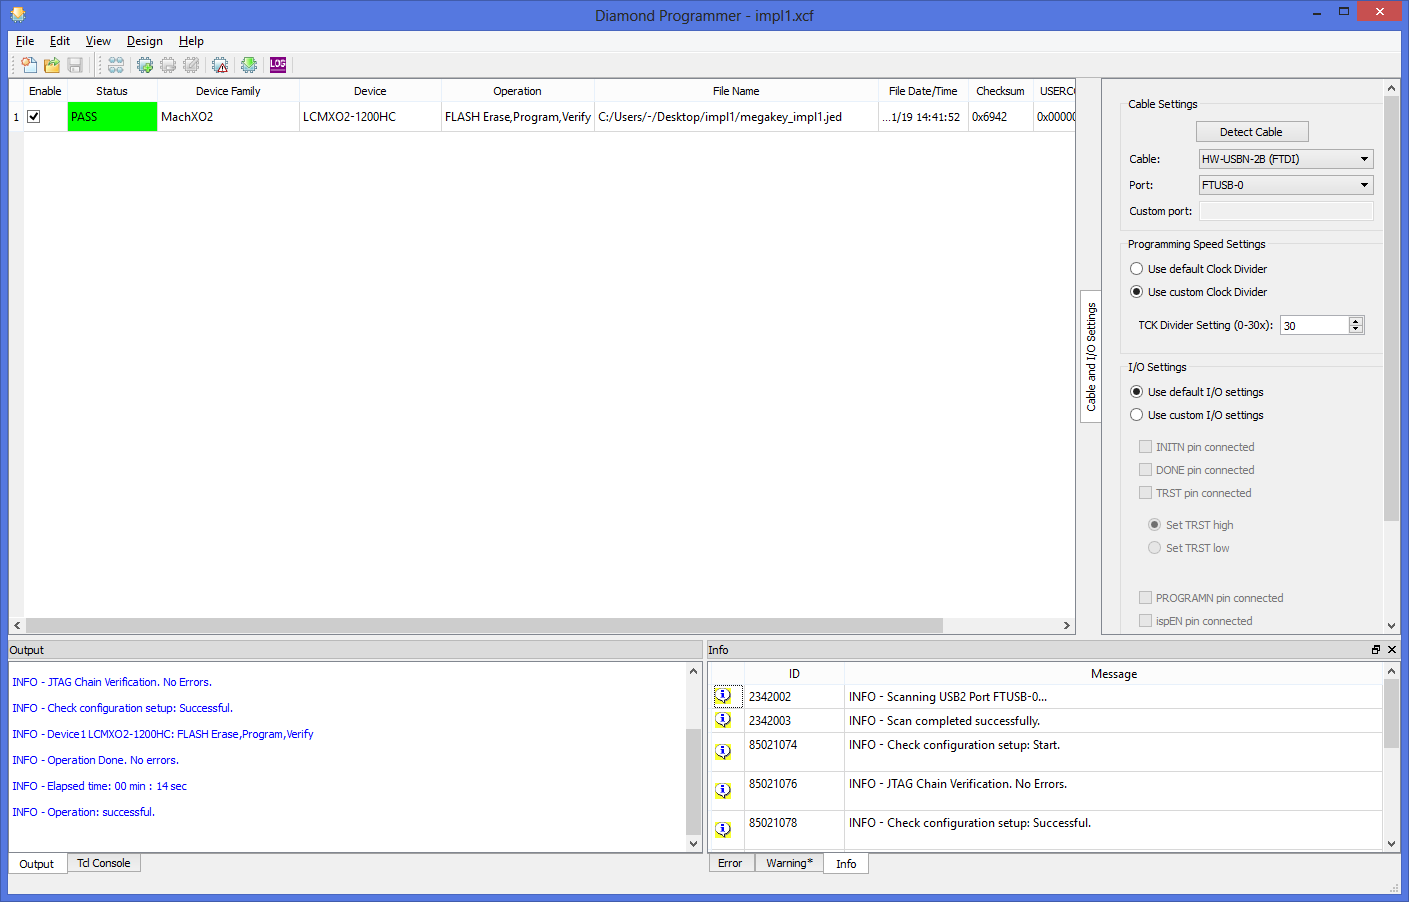
\includegraphics[width=0.8\linewidth]{images/diamond10.png}
  \captionsetup{width=0.8\linewidth}
  \caption{Step 10: Operation successful:
           You have now successfully flashed the MEGA65 keyboard.
           If you wish you can save the project now for later use.}
  \label{fig:diamond10}
\end{figure}


\section{Flashing the MAX10 FPGA on the MEGA65's Mainboard with INTEL QUARTUS}

If you choose to proceed, you will need a TEI0004 - Arrow USB Programmer2 module with TEI0004 driver installed
and a functioning installation of Quartus Prime Programmer Lite Edition.  This can be done on either Windows
or Linux, but in both cases you will need to install any necessary USB drivers.
With your MEGA65 disconnected from the power, the TEI0004 must be installed on the J17 connector,
which is located between the floppy data cable and the ARTIX 7 FPGA on the Mainboard.
The micro-USB port of the TEI0004 must face in the opposite direction of the HDMI and LAN sockets, towards
the trap door.
The following image shows the correct position.

One the PCB r2 MEGA65 Mainboard all dip switches must be in the OFF. The Artix 100T main FPGA must not contain
a valid bitstream. See section "Flashing the Artix 100T main FPGA with XILINX VIVADO" on how to erase bitstream
from ARTIX 100T.

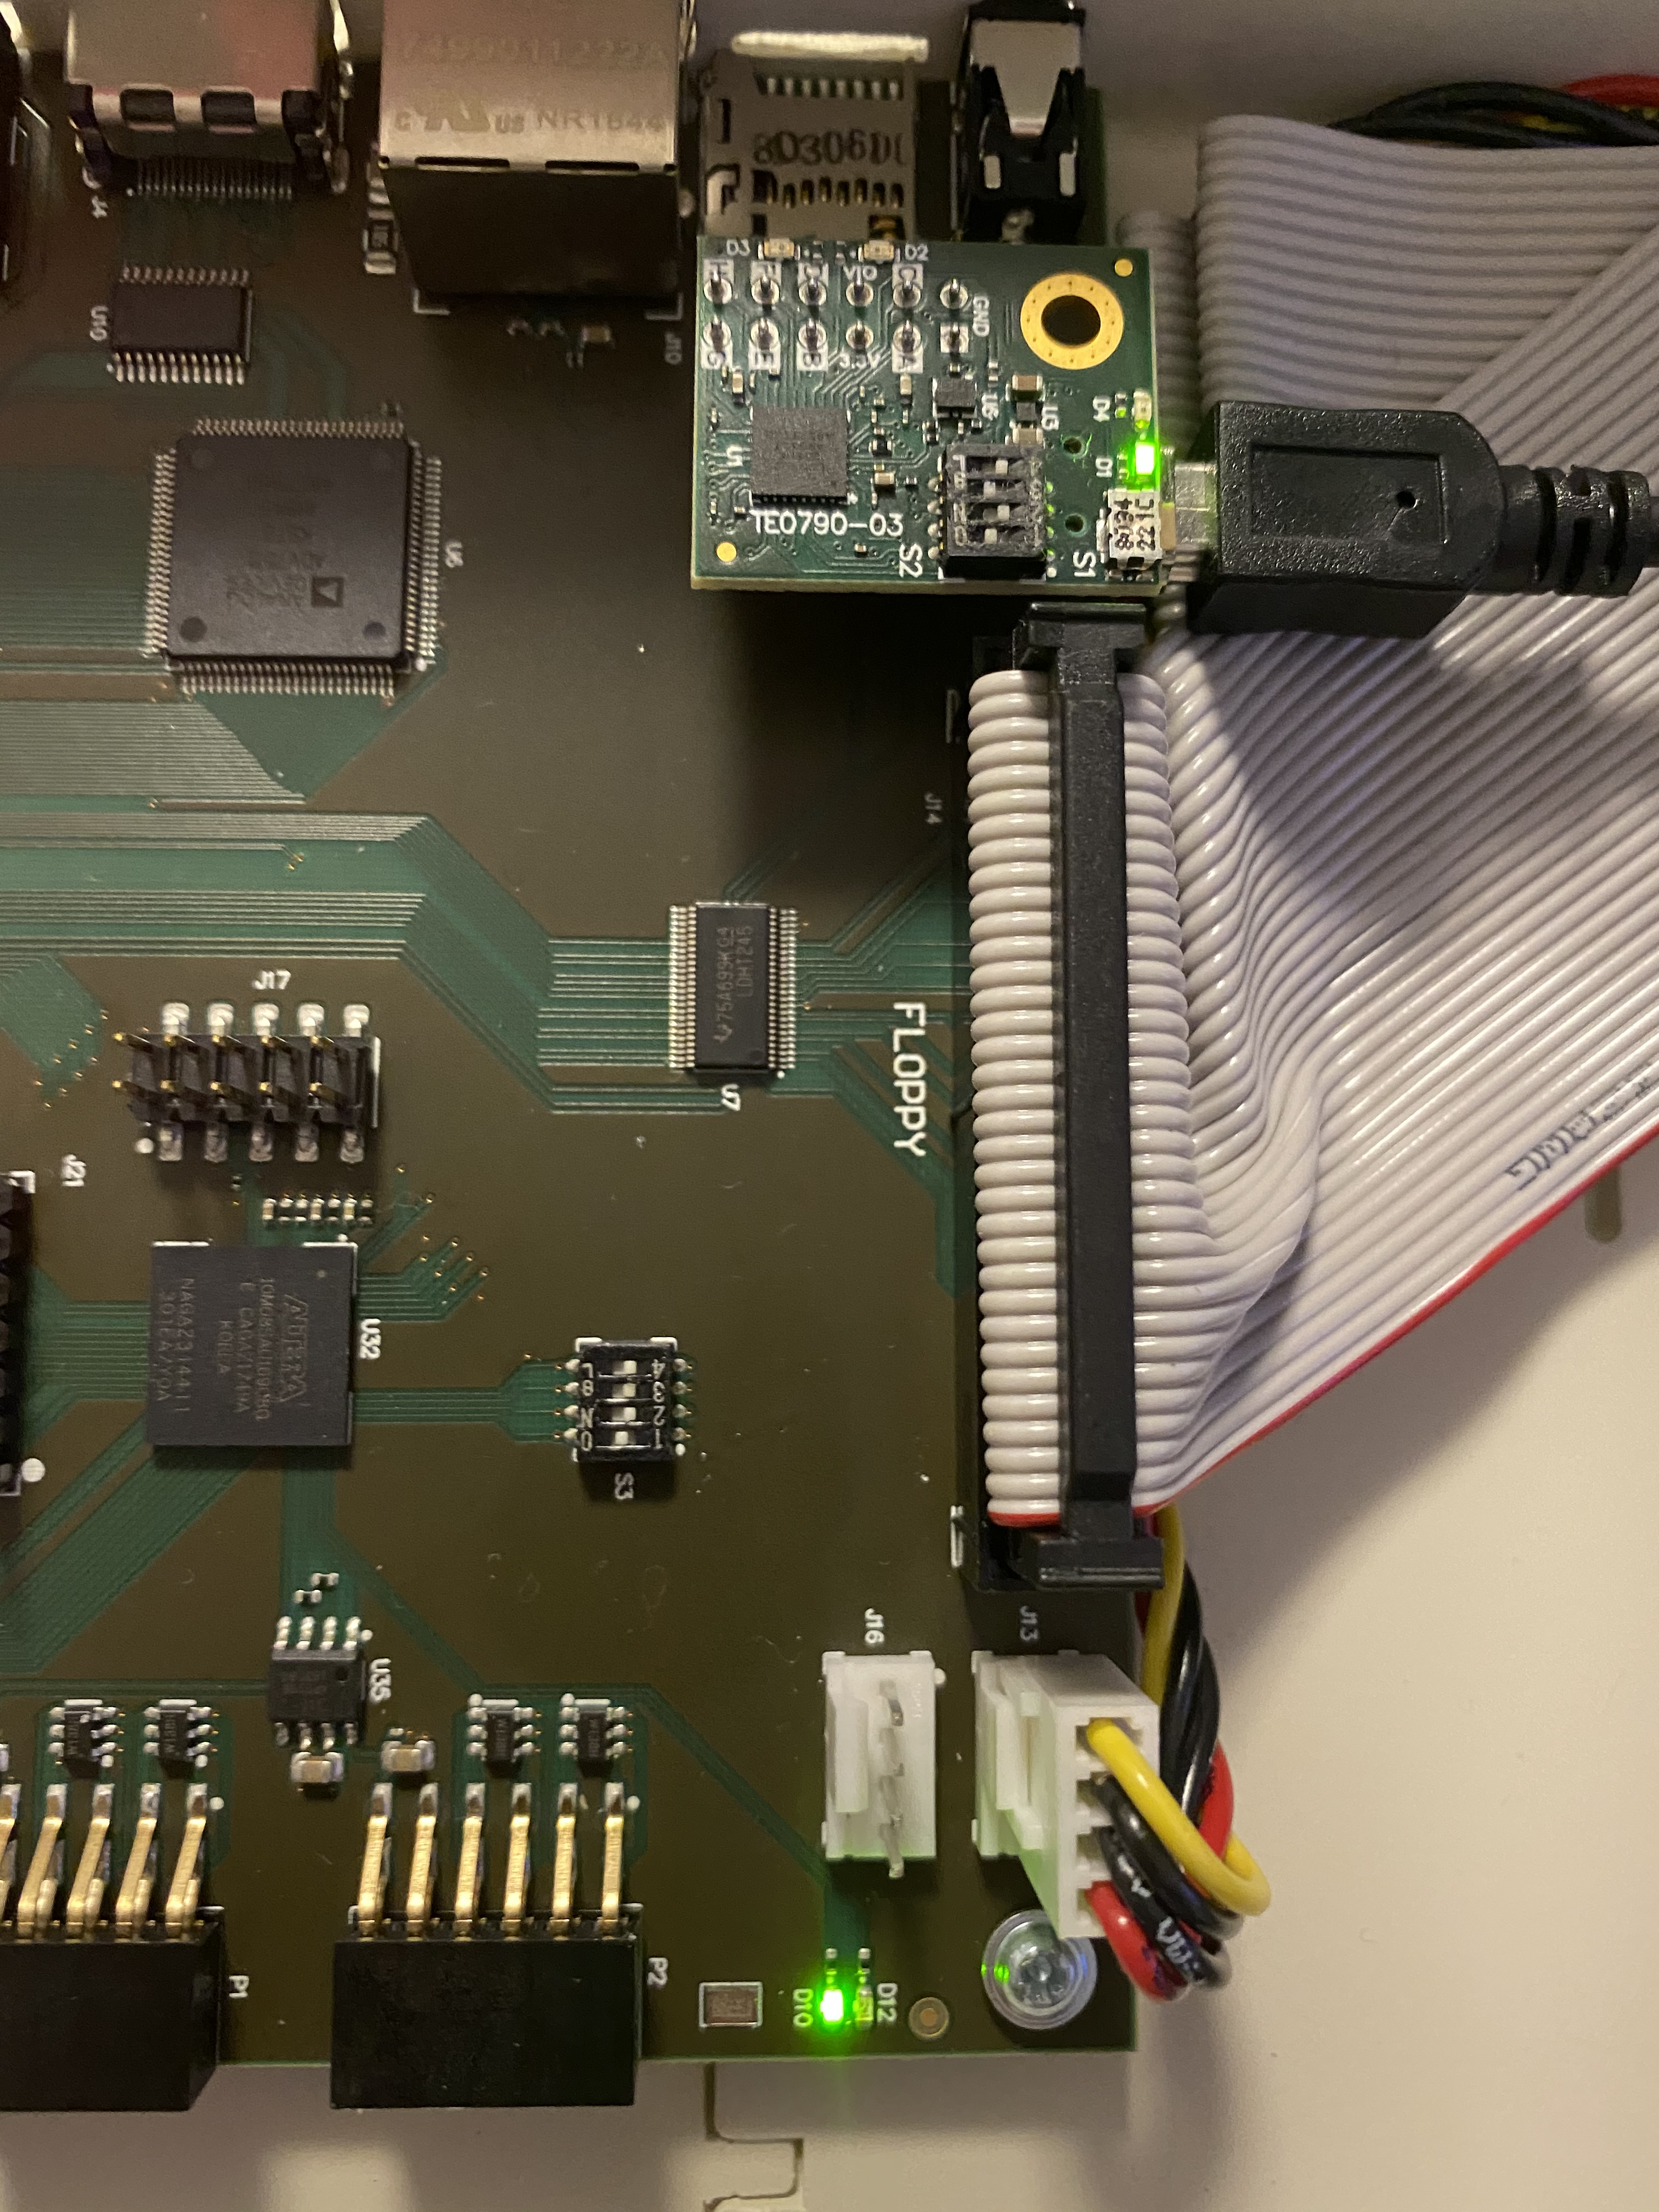
\includegraphics[width=\linewidth]{images/jtag_detail_05.jpg}

Connect your non-8-bit computer to the FPGA programming device using a micro-USB cable.
Open Quartus Prime Programmer Lite Edition, which can be downloaded from the Internet.

\begin{figure}[H]
  \centering
  
\includegraphics{images/max10_01.png}
  \captionsetup{width=0.8\linewidth}
  \caption{Step 1: Open Quartus Prime Programmer Lite Edition:
           Click the "Hardware Setup" button in the top left corner of
           the Quartus Prime Programmer window.}
  \label{fig:max10_01}
%\end{figure}

\vspace{5mm}

%\begin{figure}[H]
  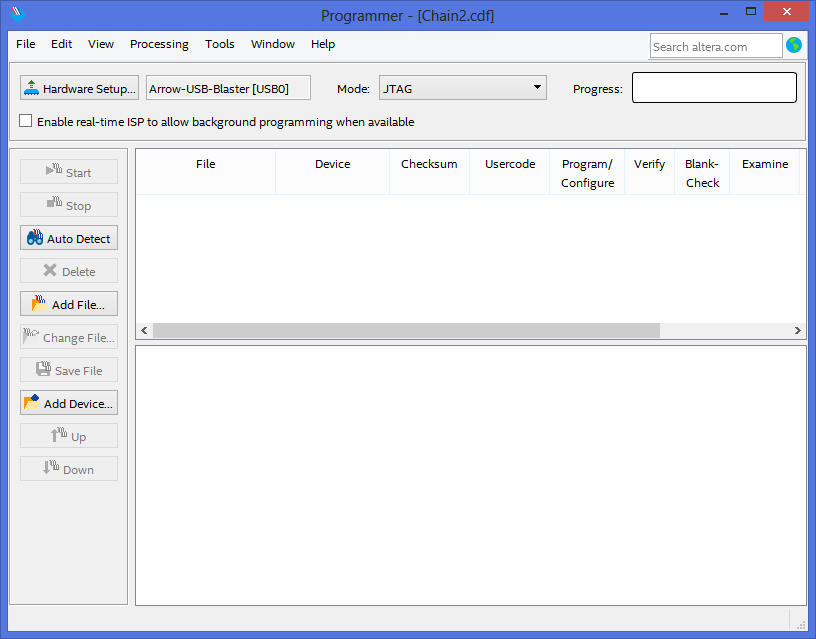
\includegraphics[width=0.8\linewidth]{images/max10_02.png}
  \captionsetup{width=0.8\linewidth}
  \caption{Step 2: Enter Hardware Setup:
           In the newly appeared window under "Currently selected
           hardware" choose "Arrow-USB-Blaster".
           If "Arrow-USB-Blaster" does not appear, verify cable and
           drivers being correctly installed.}
  \label{fig:max10_02}
\end{figure}


\begin{figure}[H]
  \centering
  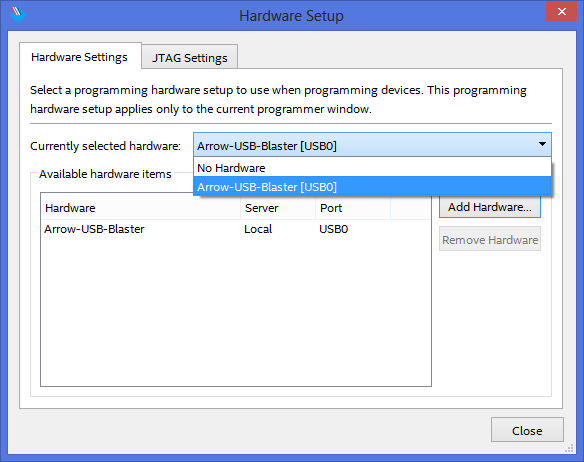
\includegraphics[width=0.8\linewidth]{images/max10_03.png}
  \captionsetup{width=0.8\linewidth}
  \caption{Step 3: Select Arrow USB-Blaster:
           Click the "Add File" button from the left row and choose the
           latest ".pof" file. Then click "Open".}
  \label{fig:max10_03}
\end{figure}


\begin{figure}[H]
  \centering
  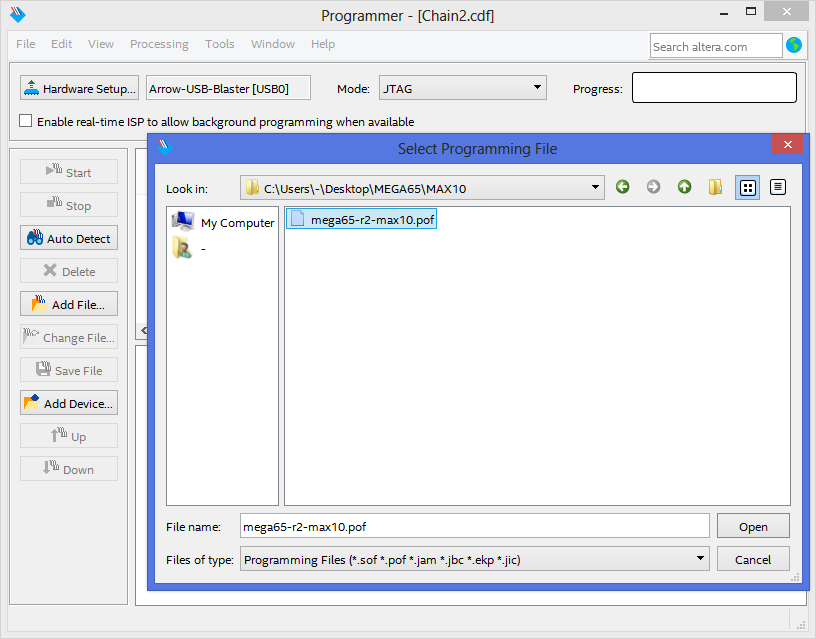
\includegraphics[width=0.7\linewidth]{images/max10_04.png}
  \captionsetup{width=0.7\linewidth}
  \caption{Step 4: Select Programming File:
           Tick at least the three boxes under "Program/Configure".
           Also enabling all boxes under "Verify" and "Blank-Check"
           will make the process more reliable.}
  \label{fig:max10_04}
%\end{figure}

\vspace{5mm}

%\begin{figure}[H]
  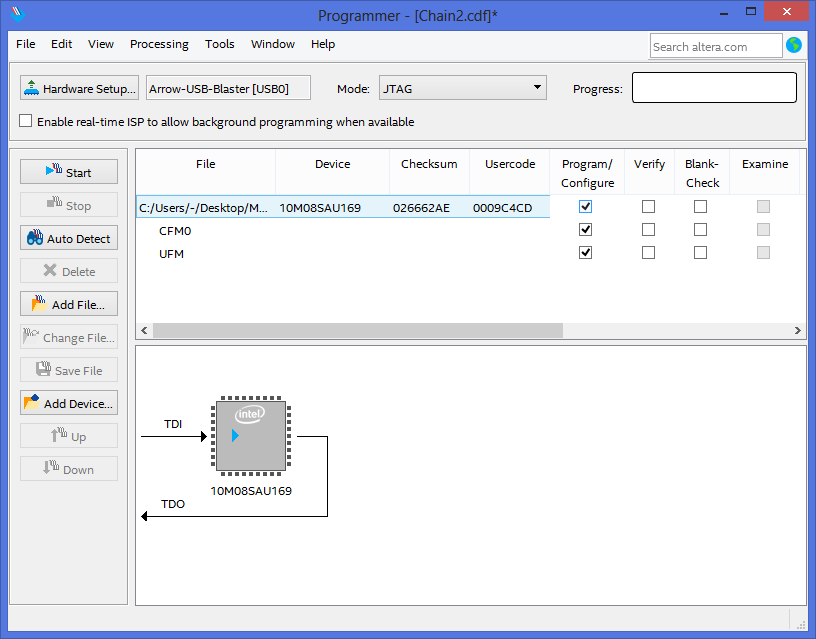
\includegraphics[width=0.7\linewidth]{images/max10_05.png}
  \captionsetup{width=0.7\linewidth}
  \caption{Step 5: Select Program/Configure Options}
  \label{fig:max10_05}
\end{figure}

While keeping the Reset-Button pressed, switch the MEGA65 computer ON.
The keyboard will go into "Police Mode" (blue and red blinking LEDs).
If it does not, the ARTIX 100T is not empty - restart the whole process.

Now click on "Start" in the left row of buttons. The progress bar in
the top right corner should quickly go to 100 percent and turn green.
You have now successfully updated your MAX10 FPGA!

If you receive an error message instead, make sure the ARTIX 100T
bitstream has been erased and you did not release the reset-button on
the MEGA65 before - switch off the MEGA65 and restart this step.

\begin{figure}[H]
  \centering
  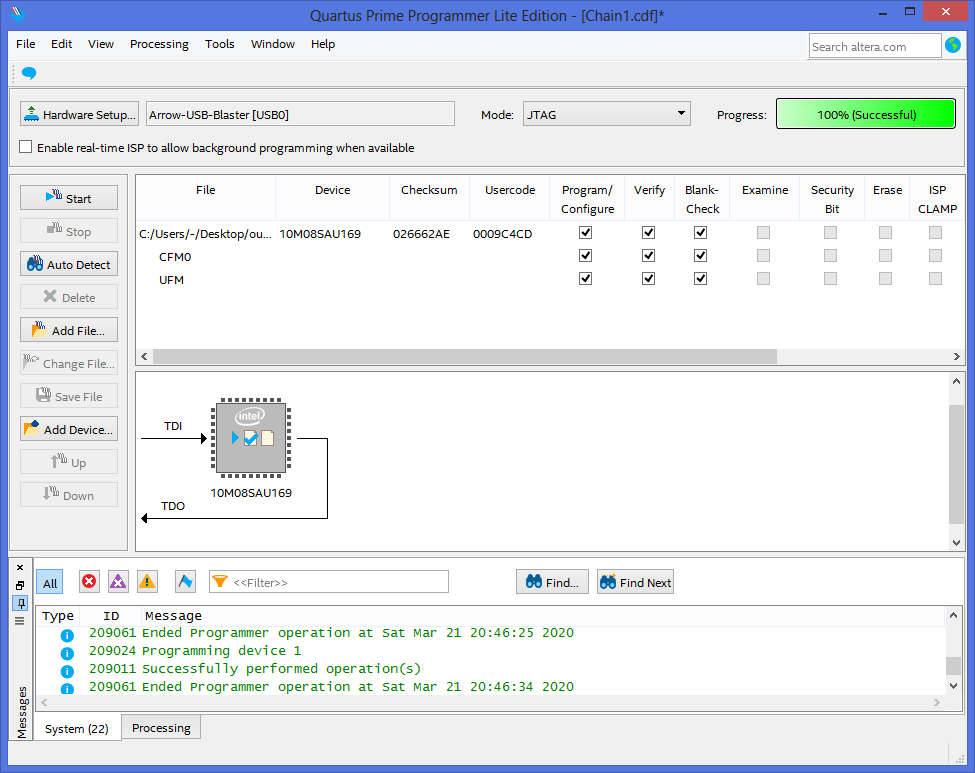
\includegraphics[width=0.8\linewidth]{images/max10_06.png}
  \captionsetup{width=0.8\linewidth}
  \caption{Step 6: Programming successful}
  \label{fig:max10_06}
\end{figure}

